%% Bachelor Thesis Template of Xidian Uniersity
%%   for using XDBAthesis package with LaTeX
%%
%% Created by Xue-Jilong(xuejilong@gmail.com)
%%
%% template.tex v0.1, 2011/03/21


\documentclass[xetex,adobefonts,master]{XDBAthesis}
% 选项说明:
% dvipdfm  使用 dvipdfm(x) 生成最终的 PDF 文档 (缺省设置)
% dvips    使用 dvips 生成最终的 PS 文档
% pdftex   使用 pdfLaTeX 生成最终的 PDF 文档
% xetex    使用 XeLaTeX 生成 PD F文档
% adobefonts 使用 Adobe 中文字体
% winfonts 使用 Windows 中文字体
% master   用于生成硕士学位论文

% 图形文件的搜索路径
\graphicspath{{chapter-utf8/}{figures/}}

\begin{document}
%%----------------- 封面部分 ----------------- %%
    \schoolnumber{1203121619}
    \title{基于压缩后缀数组的空间高效}{短读比对算法}   %%题目超过14个字把剩下的放到第二个空
    \entitle{Space-efficient Short Read Alignment with}{ Compressed Suffix Array}   %%题目超过14个字把剩下的放到第二个空
    \major{计算机软件与理论}
    \author{李双江}
    \advisor{霍红卫~~教授}
    \date{2014年11月}
    \majorclass{计算机科学与技术}
    \degreeclass{工科}

    \identifier{10701} %%学校代码
    \classnumber{TP301.6} %%分类好
    \classification{公开}
    \maketitle
    \makethemename
    \makeenthemename
%%----------------- 前言部分 ----------------- %%
    \frontmatter
    \pagestyle{empty}
    \begin{center}
\heiti\zihao{3}西安电子科技大学\\[5mm]
	学位论文独创性(或创新性)声明
\end{center}\vspace{1cm}

\songti\zihao{-4}秉承学校严谨的学分和优良的科学道德,本人声明所呈交的论文是我个人
在导师指导下进行的研究工作及取得的研究成果。尽我所知,除了文中特别加以标注
和致谢中所罗列的内容以外,论文中不包含其他人已经发表或撰写过的研究成果;
也不包含为获得西安电子科技大学或其它教育机构的学位或证书而使用过的材
料。与我一同工作的同志对本研究所做的任何贡献均已在论文中做了明确的说明
并表示了谢意。

申请学位论文与资料若有不实之处,本人承担一切相关的法律责任。\\[3mm]

	本人签名:\rule{2.6cm}{0.75pt}  \hspace{3cm}  日期\rule{3cm}{0.75pt}\\[2cm]
	
\begin{center}
\heiti\zihao{3}西安电子科技大学\\[5mm]
	关于论文使用授权的说明
\end{center}\vspace{1cm}

\songti\zihao{-4}本人完全了解西安电子科技大学有关保留和使用学位论文的规定,即:研究
生在校攻读学位期间论文工作的知识产权单位属西安电子科技大学。学校有权保
留送交论文的复印件,允许查阅和借阅论文;学校可以公布论文的全部或部分内
容,可以允许采用影印、缩印或其它复制手段保存论文。同时本人保证,毕业后
结合学位论文研究课题再撰写的文章一律署名单位为西安电子科技大学。(保密的
论文在解密后遵守此规定)

本学位论文属于保密,在\rule{6mm}{0.75pt}年解密后适用本授权书。\\[3mm]

	本人签名:\rule{2.6cm}{0.75pt}  \hspace{3cm}  日期\rule{3cm}{0.75pt}\\[3mm]

	导师签名:\rule{2.6cm}{0.75pt}  \hspace{3cm}  日期\rule{3cm}{0.75pt}           

    
\begin{abstract}

新一代基因测序技术(NGS)的出现使得测序成本飞速下降,随之而来的是大量的短读
需要更快速准确的比对程序来处理。第一代基于散列表技术的序列比对算法如MAQ等
能够快速准确的完成比对工作,但其不支持gap比对的特性使得在短读序列(short reads)
过长导致indel出现频繁时,比对的精度也随之下降。另一方面,近年来压缩索引(BWT,CSA,FM-index)
领域的相关研究使得在较小内存中索引人类基因组这样的大规模序列成为可能。这导致
近年来出现了很多基于压缩索引的短读比对算法,如BWA,Bowtie等。本文提出了一种基于压
缩后缀数组和后向搜索实现的近似匹配的算法来实现短读比对,在比对时间和空间以及比对
精度上都取得了很好的效果。

本文提出并实现的基于压缩后缀数组的短读比对算法(CSAA),采用了压缩后缀数组
的后向搜索来做近似匹配。通过引入搜索树,CSAA支持完全的gap比对。另一方面
CSAA在搜索树上使用了一种类似堆的优先堆数据结构,使得搜索树上的搜索空间大大
下降,而且每一次的搜索方向都能保证是最优的。最后结合罚分机制以及$difference$
距离,定义seed等方法,进一步降低搜索空间,提高CSAA的比对速度和精度。

CSAA的高效体现在两个方面,一是空间高效的索引方法。二是高效的近似匹配方法,包括
后向搜索,seed策略和多线程比对技术的利用。本文采用了增量法进行压缩后缀数组索引
的构建,从而跳过后缀数组的构建,降低了对内存的需求。而在比对时,seed的引入使得
在比对短读的前几十个核苷酸就可以放弃大部分无效的搜索方向。多个短读比对的相互
独立使得并行化成为可能,CSAA使用多线程时可以获得数倍的加速优势,可以根据计算
机的cpu核数指定多个线程,以取得最优的比对速度。


CSAA支持单端和双端序列比对,以Fastq格式输入,输出为标准的SAM(Sequence Alignment Map)
格式。

\keywords{短读比对,序列比对,压缩索引,压缩后缀数组}

\end{abstract}

\begin{englishabstract}

\setlength\parindent{0em}

\vspace{2ex}
Nowadays,decreasing cost and better accessibility of next generation sequencing methods
have produced a large amount of short reads whic is calling for the development of fast
and accurate read alignment programs.A first generation of hash-table based methods has
been developed,including MAQ,which is accurate,feature rich and fast enough to align short
reads from a single individual.However,MAQ does not support gapped alignment of longer reads
where indels may occur frequently.On the other hand,recent experimental studies on compressed
indexs(BWT,CSA,FM-index)have confirmed their practivality for indexing very long strings such
as human genome in the main memory,and many alignment method based on compressed index have
been developed,for example,BWA.In this paper we show how to build a software called CSAA that
exploits a CSA index of reference sequence,and perform well on alignment speed and accuration.

\vspace{2ex}
We proposed and implemented Compresses Suffix Array Alignment(CSAA),a new short read alignment
tool that is bases on backward search with compressed suffix array,to align short reads to a
large reference such as human genome.CSAA use a seach tree on multiple proximate sequences to
support mismatch and gapped alignment,CSAA also introduced a heap like structure to decrease
search space on seach tree.Finally,with the help of penalty strategy and seed,CSAA achieved
similar accuracy and faster speed than MAQ.


\vspace{2ex}
CSAA has two advantage. On one hand,increment CSA construction algorithm has beeb used in
CSAA,which directly construct CSA without SA,and use little memory to classic CSA construction algorithm.
On the other hand,CSAA used seed strategy to speed up alignment,which can drop most of invalid
seach direction when aligning the first dozons of nucleotides of a read.Lastly,indpendency of
every short read's aligment makes parallel aligning avaliable.CSAA speed up efficiently by
adopting multi-thread.

\vspace{2ex}
CSAA supports single-end and pair-end mapping with Fastq as input format and SAM(Sequence Alignment Map)
as output format.CSAA also support multi-thread running on a multi-core machine to get a faster
alignment speed.


\englishkeywords{short reads alignment, DNA sequence alignment, comressed index, compress suffix array}

\end{englishabstract}


    \listoffigures
    \listoftables
    \cleardoublepage
\begin{symbolstable}\renewcommand{\arraystretch}{1.3}

\noindent
\begin{table}[ht]
\begin{tabular}{p{5cm}p{10cm}}
\textbf{符号}&\textbf{名称}\\
$T$ & 输入的原文本序列串\\
$T[i]$ &输入序列的第$i$个字符\\
$T_i$ &输入序列的第$i$个后缀\\
$P$ & 输入的待查询的序列串\\
$P[i]$ &输入待查训序列的第$i$个字符\\
$n$&输入原串的长度\\
$\Sigma$&字符集\\
$m$ &输入待查训序列的长度\\
$P_i$ &输入待查训序列的第$i$个后缀\\
$l_i$ &模式序列$P_i$在原序列$T$上的位置\\
$\$$ &缀在模式最后的标识字符,小于模式中所有的字符\\
$SA$ &后缀后缀\\
$SA^{-1}$ &后缀数组的逆数组\\
$SA_T$ &输入序列$T$的后缀数组\\
$CSA$ & 压缩后缀数组\\
$\Phi$&压缩后缀数组变换后的数组\\
$difference$ & 短读相似度距离\\
$seed$ & 短读的可信部分\\
\end{tabular}
\end{table}
\noindent
\clearpage
\begin{table}[ht]
\begin{tabular}{p{6.5cm}p{7cm}}
\textbf{函数}&\textbf{名称}\\
$\alpha (c)$ &序列中小于字符$c$的所有字符的个数\\
$\beta (c)$ &序列中等于字符$c$的所有字符的个数\\
$rank_0(i)$ &一个01序列上前$i$位中的所有0的个数\\
$select_0(i)$ &一个01序列上第$i$个0出先的位置\\
$rank_1(i)$ &一个01序列上前$i$位中的所有1的个数\\
$select_1(i)$ &一个01序列上第$i$个1出先的位置\\
$BackwardSearch(P,\Phi,\alpha,\beta)$ & 在压缩后缀数组上用后向搜索方法搜索模式$P$的位置\\
$ExactMatch(c,\Phi,\alpha,\beta,l_{old},r_{old})$& 在压缩后缀数组上做精确匹配$c$\\
$InExactMatch(\Phi,\alpha,\beta,P)$&在压缩后缀数组上做近似匹配$P$\\
$CalculatDifference(\Phi,\alpha,\beta,P)$&计算$P$的$difference$距离\\
$ProcedureIndel(P,\Phi,\alpha,\beta,x,heap)$&处理近似匹配序列$x$的indel\\
$CsaAlignment(\Phi,\alpha,\beta,P)$&在参考序列$T$的压缩后缀数组上比对短读$P$
\end{tabular}
\end{table}

\end{symbolstable}


\begin{abbreviation}\renewcommand{\arraystretch}{1.3}
\noindent
\begin{table}[ht]
\begin{tabular}{p{2cm}p{6cm}p{8cm}}
\textbf{缩略语}&\textbf{英文全称}&\textbf{中文对照}\\
SA &Suffix Array &后缀数组\\
CSA & Compressed Suffix Array &压缩后缀数组\\
CSAA & Compressed Suffix Array short reads Aligment tool & 压缩后缀数组短读比对工具\\
BWT & Burrows-Wheeler transform&BW变换\\
BWA & BWT short reads Alignment tool & BWT短读比对工具\\
indel & insert and delete &插入和删除\\
\end{tabular}
\end{table}
\end{abbreviation}

    \tableofcontents

%%----------------- 正文部分 ----------------- %%
    \mainmatter
    \pagestyle{content}
    \chapter{绪论}
\label{chap:introduction}

\section{研究背景及意义}

DNA(脱氧核糖核酸)是生物遗传信息的载体,其双螺旋结构的两个链互相补充,构成稳定结构。其中每个链都含有完备的遗传信息,这些
遗传信息体现在构成DNA链的四种碱基——腺嘌呤(A),胸腺嘧啶(T),鸟嘌呤(C)和胞嘧啶(G)的排列顺序上。在现代生物学研究中,
为分析DNA的遗传表达等特性,需要特定对物种DNA进行测序。早期的sanger测序作为第一代测序手段在人类基因组计划中起到了巨大的作用。

随着生物学,医学等相关科学的发展,新的DNA测序技术不断涌现,其中,以Illumina/Solexa为代表的NGS(Next-Generation Sequencing technologies)
技术以其低廉的测序成本和便捷快速的特点成为当前的主流DNA测序技术。基于这一新技术实现的测序机器每台工作一天就能产生数十亿的
短读序列(short reads)\cite{metzker2009sequencing}。NGS测序技术一般应用于两类测试场景,重测序(Resequencing)
和从头测序(de novo sequencing),这也对应着产生了DNA分析领域的两个最核心的研究问题:比对(alignment)和重组(assembly)。
若测序的目标物种的基因序列之前还从未被测序过,那么从头测序就是研究的第一步,这需要关注把短读以最优方式连接起来。若测序目标
物种已经完成了测序,那么重测序关注的问题是如何把短读序列映射到已知的同物种基因组上,从而分析同源生物的个体基因差异,这个过
程就是本文关注短读比对(short read alignment)。由于每一次测序实验都会得到大量的短读(short reads)序列(5亿到20亿个),同时生物
个体基因之间的差异会导致基因序列存在差异,短读映射面临着基因的近似比对和快速高效比对两个难题。本文即提出一种基于压缩后缀
数组索引算法的快速高效比对算法来解决这两个问题。

重测序得到的短读序列中每一个短读一般不超过1000个碱基(大多数情况下都是20到100个碱基的长度),但一次测序实验中短读数量都
会超过一千万个。参考序列是已经经过准确测序,重组后的已知基因组序列,比如人类基因组序列就是合并出来的总长达2.8G的DNA序列。
出于医疗,身份鉴别等原因会对某个具体的人进行再次DNA测序,这就是DNA重测序,此时测序得到的大量短读序列分析的第一步就是把
这些短读映射到参考序列上,对人类而言,大多都是映射到人类基因组序列上,也可以映射到一个人工合成的参考序列上。映射的过程是
对每一个短读在参考序列上查找的过程,即要在参考序列上找到一个合适的位置,使得从这个位置开始,短读是参考序列的一个子串。

综上所述,短读序列的比对问题可以抽象为一个模式查找问题:给定一个共有$m$个模式的模式集合$P=\{P_1,P_2\ldots P_m\}$,每个
模式的长度已知分别为$l_1,l_2\ldots l_m$,已知一个长为$n$的参考序列$T$,求得一个集合$S=\{s_1,s_2\ldots s_n\}$使
得$P_i=T[s_i\ldots s_i+l_i-1]$。这个查找的过程即为短读到参考序列的比对映射。其中参考序列$T$和短读序列$P_i$都是由DNA测序
中常用的碱基字符$\{A,T,C,G,N\}$构成的。

\section{研究现状}
为实现快速且准确的短读序列映射,近年来出现了很多比对算法。所有这些算法都可以分为两类,一类是通过对短读序列使用散列表等方法建
立短读序列的索引,之后遍历整个参考序列。另一类是为参考序列建立索引,之后再对每个短读进行独立的比对。

第一类比对算法的代表是MAQ,ZOOM,SHRiMP等。MAQ\cite{li2008mapping}基于散列技术,结合短读中每一个核苷酸的测序质量分数,实现了
无空位(ungapped)比对。ZOOM\cite{lin2008zoom}使用了space seeds技术,提高了比对的精确率。而SHRiMP\cite{rumble2009shrimp}则结合space seeds''
和smith-waterman算法得到了更高的精确率。

第二类算法为参考序列建立索引,通过索引后的数据可以实现快速的比对。如SOAP,WHAM,BFAST等。SOAP\cite{li2008soap}使用seeds技术
和一个散列查询表加速比对,且可以处理较少的空位比对。WHAM\cite{li2012wham}对参考序列建立散列表,先通过散列表查找潜在的比对
位置,再进一步比对确定最终结果。BFAST\cite{homer2009bfast}则通过
为参考序列建立多个索引来提高精确度。这几种方法使用的索引方法都需要很大的内存空间,所以比对时空间需求很大,尤其是在用类基因
组这样的较大序列作为参考序列时。在第二类方法中以SOAP2,Bowtie,BWA为代表的基于BW变换(Burrows-Wheeler transform,BWT)\cite{ferragina2005indexing}来创建参考序列
索引的方法具有很大的空间优势。Bowtie\cite{langmead2009ultrafast}使用BWT建立索引,采用回溯递归
的搜索方法,再结合双端搜索实现了高速,空间高效的比对,是目前最快的比对软件之一,但缺陷是不能实现空位(gap)比对。BWA\cite{li2009fast}
也是基于BWT的一种比对算法,比对速度较Bowtie慢,但可实现空位比对。SOAP2\cite{li2009soap2}使用了bidirectional BWT来建立参考序列
的索引,比对速度和Bowtie相当。基于BWT的这些方法都使用了后向搜索方法\cite{lippert2005space}来加速查询。后向搜索可以在$O(m)$时间内实
现长为$m$的字符串的计数查询,以及$O(m\log n)$时间复杂度的query查询。利用后向搜索的性质,Bowtie实现了基于
回溯法的非精确匹配算法,而BWA则采用前缀树搜索的方法实现非精确匹配。在实现非精确匹配的基础上,加上一些打分机制,既实现了短读
序列到参考序列的匹配。

\section{本文的主要工作}

本文提出一种采用压缩后缀数组(Compressed Suffix Array,CSA)建立
索引\cite{grossi2005compressed},实现短读比对的算法:CSAA(csa alienment)。这一算法采用的是CSA的后向搜索特性,同时还使用了
优先队列来保存所有可能的匹配位置,并为每个可能的匹配位置打分,在匹配过程中,通过分支限界抛弃所有低分搜索方向,降低搜索空间,
同时保证匹配结果最优。按照上一节中对短读比对算法的分类,该算法属于对参考序列进行索引的比对算法。

本文总共六章,按照以下形式组织。

第一章是全文简介,主要介绍本文所研究的课题,研究背景及其意义。并对国内外研究现状做了简单介绍。突出本文所提出的CSAA的研究意义。

第二章预备知识详细介绍了本文中要用到的一些先验知识,包括压缩索引和序列比对两部分。前者重点介绍索引,自索引,压缩索引的相关概念,
后者是本章的重点,详细介绍了序列比对的相关知识,比对数据的构成,比对的评判标准等。

第三章是本文应用的索引算法压缩后缀数组的介绍,内容包括了压缩后缀数组的原理,构建算法,RRR数据结构的原理和实现等。并且之后还给出
了本文中应用的搜索算法,后向搜索的时间分析和空间分析,作为之后CSAA实现的基础。

第四章是本文的核心,主要介绍了我们提出的序列比对算法比对原理,比对过程,以及对时间,空间占用的分析。首先在第一小节给出了一个简
单的基于压缩后缀数组的精确比对算法,接着在第二小节我们在精确比对的基础上给出了一个理论的递归的近似比对算法。之后我们分析了
近似比对算法的时间和空间需求,提出了分支限界的思想,通过$difference$距离和罚分机制实现了分支限界,最后我们提出了一个实践中
可行的化递归为迭代的优先堆数据结构,提出了最终的比对算法。

第五章是在第四章提出的算法的基础上给出了CSAA的实现方法。重点描述了在应用领域如何去提高比对的时间效率,空间效率,比对精度等指标。
描述了空间高效的索引方法的应用,多线程的应用,seed的应用以及双端比对的实现等概念。每一个改进我们都在随后给出了实验测试效果。最后
在第五章结尾,我们给出了CSAA和BWA,bowtie,MAQ等的对比测试。验证了CSAA在某些方面的优越特性。

第六章是对全文的总结,归纳了本文提出的算法的相关特性。同时提出了CSAA的一些不足点,以及可以改进的工作。

    %%第二章,预备知识
\chapter{预备知识}
\label{chap:predefine}
序列比对领域常用的比对方法是对短读序列或者参考序列建立索引,除了前文所提到的通常的基于散列表的索引方法之外,最常使用的就
是压缩索引算法。压缩索引一方面能对数据规模进行压缩,减少算法实现时对内存空间的需求;另一方面也起到索引的作用,加快对模式的
搜索。如前文所述,DNA数据经过处理后可以当作一个文本序列,而序列比对问题可以抽象为一个模式查找问题,因此,序列比对使用的索
引方法本质上是文本索引算法。本章将介绍文本索引算法的一些概念,同时在第二部分对DNA数据格式处理做一些简述。

\section{压缩索引}
文本索引的目的是加快模式查询的速度。模式查询问题可以表述为:给定一个长为$m$的输入模式,找出$P$在长为$n$的文本$T$中的出现位置。
在模式查询领域,KMP提出了第一个时间复杂度为$O(m+n)$的线性查询算法,空间需求只有$O(1)$,这是非索引方法所能达到的最优结果。之
后为提高查询速度所涉及的搜索算法都是基于索引的方法。当前最优影响力的索引是倒排索引,但倒排索引是一种词索引,文本$T$必须
是结构化的,可以分为词,以便构建单词集。而如DNA等数据,是没有明显的单词集的,其所查询的模式也可能出现在文本$T$的任何一个
位置,即模式串$P$可以是$T$的任意子串。而后缀数组和后缀树以及类似trie树或者自动机都可用于DNA这样的无结构文本的模式查询,这
种索引称为全文本索引(full text index)。

后缀数组和后缀树由于其所需存储空间过大,在实践应用中存在诸多限制,而压缩索引的出现就是针对全文本索引空间复杂度过高的一个解决
方案。最有名的两个全文本压缩索引就是压缩后缀数组和FM索引。这两个索引的优势还体现在其自索引性质上,即建立索引后,无需再保存
原文本$T$,CSA或者FM本身即隐含了文本$T$,这进一步使得索引的规模降到了文本的0阶经验熵。另一个问题是构建CSA或者FM时,都需要
$O(n\log n)$位的辅助空间,这使得在构建较大规模的文本(如本文中使用的人类基因组)索引时,对计算机内存的需耗很大,在常规PC上
无法完成索引构建工作,对此,Hon,Sadakane和Sung提出了逐步构建CSA和FM,再归并的方法\cite{lam2002space}\cite{hon2003constructing},
使得构造空间降低到了$O(n\log |\Sigma|)$位。

以BWT为代表的自索引算法近年来在序列比对领域多有出现,例如前文中提到的Bowtie,BWA等。本文提出的序列比对算法则使用另一种自索引
算法:压缩后缀数组(CSA)\cite{grossi2005compressed}。同BWT相比,CSA的模式查询速度更快,应用于序列比对,相应的比对速
度也会更快,提高整个比对的效率。

CSA上的模式查询使用后向搜索算法(backward searching),Sadakane已经证明,在CSA上的后向搜索实践复杂度是$O(m)$,条件是字符集满足
$|\Sigma|=O(\text{poly} \log(n))$\cite{sadakane2002succinct}。本文提出的CSAA比对算法中,序列的查询也使用的是后向搜索算法。

\section{短读序列比对}

\subsection{DNA序列格式}

在DNA序列分析领域,DNA数据一般都来自国际知名的几大DNA数据库,如GenBanki,EMBL,DDBJ等。不同的测序方法,通常得到的序列数据也会
有一些差异。对此,为方便后续处理,生物信息学定义了一些通用的序列存储格式,如Fasta,Fastq等。通常Illumina测序数据都是Fastq格式,
所以本文中实现的软件CSAA也以Fastq作为标准输入格式。

Fastq格式是DNA序列格式中常见的一种,Fastq格式的序列一般都包含有四行,第一行由'@'开始,后面跟着序列的描述信息,这点跟Fasta格式
是一样的。第二行是序列的字符表示。第三行由'+'开始,后面也可以跟着序列的描述信息,和第一行信息相同,通常可以省略。第四行是第二行序列的质量评价
(quality values,是测序的质量评价),字符数跟第二行的序列是相等的。下面是Fastq格式序列的一个序列示例。

\begin{verbatim}
@HWUSI-EAS100R:6:73:941:1973#0/1
GATTTGGGGTTCAAAGCAGTATRRRGYKKKMSTCAAATAGTAAATCCATTTGTTCAACT
+HWUSI-EAS100R:6:73:941:1973#0/1
!''*((((***+))%%%++)(%%%%).1***-+*''))**55CCF>>>>>>CCCCCCC6
\end{verbatim}

Illumina测序仪是按照荧光信号来判断所测序的碱基是哪一种的,例如红黄蓝绿分别对应ATCG,但对每个结果都是有一定的误差的。最初sanger
中心用Phred quality score来衡量该read中每个碱基的质量,既$Q=-10\lg P$ ,其中$P$代表该碱基被测序错误的概率,如果该碱基测序
出错的概率为$0.001$,则$Q=30$,30+33=63,63对应的ASCii码为“?”,则在第四行中该碱基对应的质量分数代表值即为“?”。
一般地,碱基质量从0-40,既ASCii码为从 “!”(0+33)到“I”(40+33)。这上是sanger中心采用记录read测序质量的方法,Illumina
没有完全依照sanger中心的方法来定义测序质量,而是把$P$换成了$P/(1-P)$,其他完全按照sanger的定义来做。可以看出当测序质量
很高的情况下两种形式几乎没区别,但低质量的碱基则有区别了。

在Fastq格式中还可能出现其他一些核苷酸符号,具体含义如表\ref{tab:tabatcg}所述。

\begin{table}[htbp]
    \caption{Fastq格式支持的核苷酸符号}
    \label{tab:tabatcg}
    \centering
    \begin{tabular}{ll}
        \hline\\
        核苷酸代码&意义\\
        \hline\\
        A & Adenosine \\
        C & Cytosine \\
        G & Guanine \\
        T & Thymidine \\
        U & Uracil \\
        R & G A (puRine) \\
        Y & T C (pYrimidine) \\
        K & G T (Ketone) \\
        M & A C (aMino group) \\
        S & G C (Strong interaction)\\
        W & A T (Weak interaction) \\
        B & G T C (not A) (B comes after A)\\
        D & G A T (not C) (D comes after C) \\
        H & A C T (not G) (H comes after G) \\
        V & G C A (not T, not U) (V comes after U)\\
        N & A G C T (aNy)\\
        X & masked \\
        - & gap of indeterminate length
    \end{tabular}
\end{table}

DNA序列的标准保存格式是Fastq等格式,同样的,对序列比对的输出格式,也有一个约定的标准数据格式:SAM格式。SAM的全称是
sequence alignment/map format,一般是文本形式的,也可以存为二进制形式文件,即BAM格式。SAM由头文件和map结果组成,头
文件由一行行以“@”起始的注释构成。而map结果是类似下面的文本:

\begin{verbatim}
C12FP66670 0    chr1  12805 1 42M4I5M * 0 0 TTGGATGCCCCTC...
C12FP30032 272  chr1  13494 1 51M     * 0 0 ACTGCCTGGCGCT...
\end{verbatim}

SAM文件中每个read只占一行,被tab分成了很多列,一共有12列,分别记录了:read名称,SAM标记,chromosome名称,5′端起始
位置,MAPQ(mapping quality,描述比对的质量,数字越大,特异性越高),CIGAR字串(记录插入,删除,错配信息),mate名称(
记录mate pair信息),mate的位置,模板的长度,read序列,read质量,程序用标记。

本文中重点关注的是第三列,chrome名称,以及第四列,起始位置。通常作为参考序列的基因组是由多条染色体构成的,比对程序
需要得到read在哪一条染色体上,以及在改染色体上的位置,即5'端起始位置。

\subsection{单端测序和双端测序}
目前的测序方法中,如Solid,都有单端测序(Single-read)和双端测序(Paired end)之分。二者再测序方法上不同,得到的测序数据也有一些
差异。主要区别在于文库的建立上。

无论是单端测序还是双端测序,第一步都是对DNA分子进行切割,这是通过切割酶来实现的。切割后,大DNA分子被切割成长为300bp左右的短
序列(fragments)。测序第二步是增值,通过对这些短序列进行复制,增值,提高DNA分子数量。第三部是加入引物,开始测序。单端测序时
只在DNA短序列分子的一端加上引物,然后依次读取核苷酸,直到读完一个read。通常一个read长为80到1000bp,读取核苷酸时,因为越往后
读取错误率越高,所以一般read序列也是越往后,可靠性越低。双端测序时,会在DNA短序列两端都加上引物,然后分别读取核苷酸。所以,
双端测序得到的是一个DNA短序列分子的两个read,这两个read读取的是DNA链的两个不同的链,并且因为只读取两端的前100bp左右的核苷酸,
所以,这两个read序列并不一定重合,二者之间有一定的距离(distance),distance的长度为短序列(fragment)的长度减去两个短读序列的
长度之和。反映到在参考DNA序列上,distance为两个序列映射位置之差的绝对值。

\subsection{DNA序列的预处理}
DNA序列的输入格式是Fastq,需要首先对其做一些预处理工作,将序列数据转成结构化的文本数据,以便使用CSA建立索引和比对。预处理
包括两部分数据的处理。处理方法类似。

首先建立索引时需要把参考序列处理成一个单串,因为参考序列会有多条序列组成,需要把这多条序列连接成一条序列,然后再建立索引。
预处理参考序列时要保存序列的辅助信息,这需要一个辅助的数据结构来完成。此外因为比对时的输入短读序列也需要保存其辅助信息,
所以预处理reads时一样要把核心的碱基序列提取出来,并用辅助数据结构保存reads的辅助信息。

\subsection{短读比对的过程}
短读序列比对是通过在一个参考序列中搜索一个模式,使得该模式和给定的短读序列尽量相似的过程。在比对的过程中,如果参考序列和
短读序列的两个核苷酸相同,称为一个匹配(match),如果不相同称为一个错配(mismatch)。错配一般有替换(substitute),插入(insert),
删除(delete)三种,后两者本质上都是让一个核苷酸和一个空位相匹配,所以插入和删除统称为空位比对(gap alignment)。如图\ref{fig:mismatch}
中,两个DNA序列的一个比对,图中上部分是参考序列的一个片段,下半部分是一个短读。这个匹配中,可以看到有多个错配(图中蓝色标记),
两个替换失配:G替换为C和A替换为T;还有两个gap匹配,C匹配一个gap,gap匹配一个T。在短读比对中,插入操作定义为在短读上插入一个
gap,而删除操作则定义为在参考序列上插入一个gap,这和在短读上删除一个核苷酸是等价的。由于参考序列建立索引后直接在参考序列上插
入gap是难以直接实现的,所以参考序列上的gap插入可以用read上的删除替代。

\begin{figure}[htbp]
    \centering
    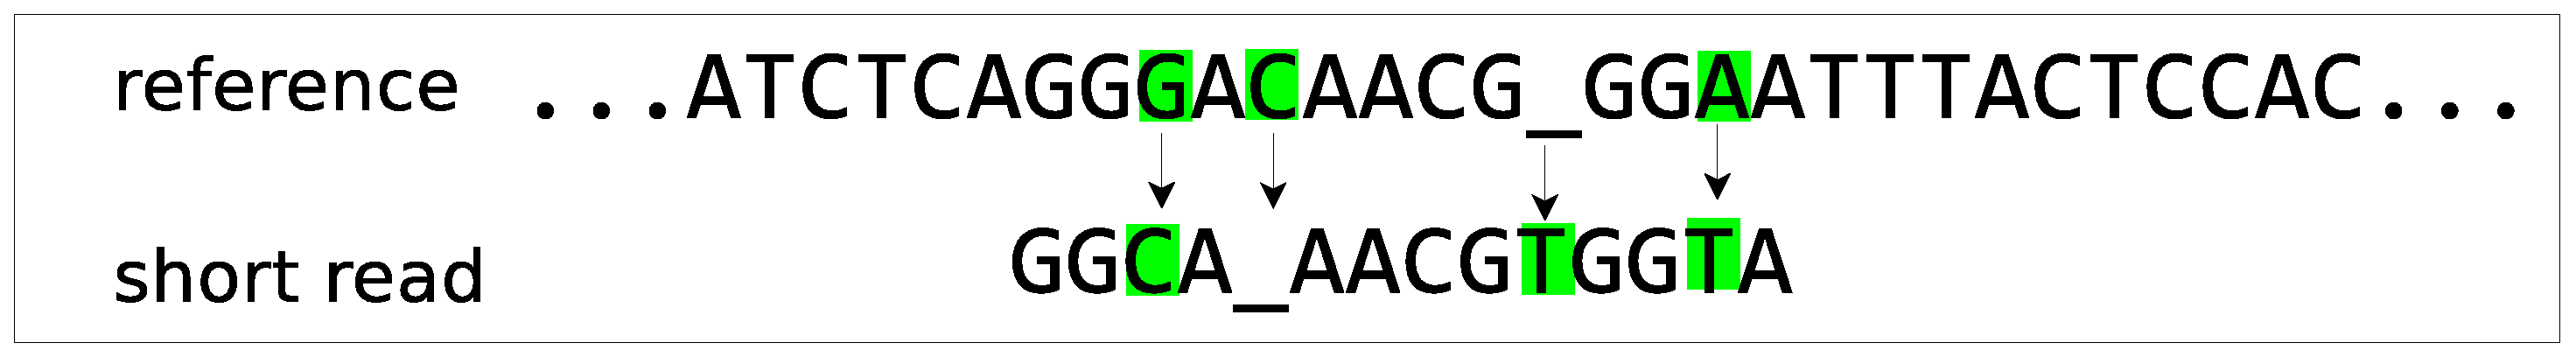
\includegraphics[width=0.9\textwidth]{mismatch.eps}
    \caption{短读比对示例} \label{fig:mismatch}
\end{figure}

\section{本章小结}
本章分为两个部分,对本文用到的一些先验知识做了一些简述。第一部分简述了索引,全文算引,自索引等概念,并对本文要用到的
索引算法:压缩后缀数组做了简介,描述了其特性,以及后向搜索。第二部分是对生物信息学领域序列
比对的一些基本概念的解释。包括DNA序列数据格式和单端测序,双端测序的概念。

    \chapter{压缩后缀数组的实现}

\section{后缀数组和压缩后缀数组}
压缩后缀数组(CSA)是由Grossi和Vitter\cite{grossi2005compressed}最早提出的第一种实现全文索引的压缩索引数据结构,是对后缀数组(SA)
\cite{manber1993suffix}占用空间过大的改进,并且实现了自索引特性。

设长为$n$的文本序列$T$,字符集为$\Sigma$,本文中将假设$T$有一个特殊的结尾符号$\$$,$\$$不在$\Sigma$中并且字典序小于$\Sigma$
中的所有符号。假设$T$存储在一个数组$T[0\ldots n-1]$中。对任何的整数$i$,假设
\begin{itemize}
    \item $T[i]$为$T$中从左往右0开始的第$i$个字符;
    \item $T_i$为$T$的第$i$个后缀,即$T_i=T[i]T[i+1]\ldots T[n-1]$。
\end{itemize}

$T$的后缀数组$SA[0\ldots n-1]$定义为
$T$的$n$个后缀按字典序排序后的序列,由$\{0,1,\ldots, n-1\}$的一个排列构成,满足$T_{SA[0]}<T_{SA[1]}<\ldots<T_{SA[n-1]}$。即$SA[i]$
表示$T$的$n$个后缀中第$i$小的后缀的开始位置。如表\ref{tab:tabsuffix}所示。后缀数组占用空间$n\log n$,给定文本$T$和其后缀数组
$SA[0\ldots n-1]$,$T$中的任何模式$P$可以在$O(|p|\log n+occ)$时间复杂度内求出其出现位置\cite{manber1993suffix},并且不需要
读原文本$T$。其中$occ$是模式的出现次数。

对于任意的整数$i \in [0\ldots n-1]$,定义$SA^{-1}[i]=j$使得$SA[j]=i$,很明显$SA^{-1}[i]$为$T_i$在$T$的所有后缀中的排名,即
$T$的后缀中比$T_i$小的后缀的数量。

\begin{table}[htbp]
    \caption{$acaaccg\$$的后缀数组和$\Phi$数组}
    \label{tab:tabsuffix}
    \centering
    \begin{tabular}{lllllll}
%        \hline\\
        \toprule
        $i$&$T[i]$&$T_i$&$SA[i]$&$T_{SA[i]}$&$\Phi[i]$&$T[SA[i]]$\\
%        \hline\\
        \midrule
        0&a&acaaccg\$&7&\$&2&\$\\
        1&c&caaccg\$&2&aaccg\$&3&a\\
        2&a&aaccg\$&0&acaaccg\$&4&a\\
        3&a&accg\$&3&accg\$&5&a\\
        4&c&ccg\$&1&caaccg\$&1&c\\
        5&c&cg\$&4&ccg\$&6&c\\
        6&g&g\$&5&cg\$&7&c\\
        7&a&\$&6&g\$&0&g\\
%        \hline
        \bottomrule
    \end{tabular}
\end{table}

\begin{equation}\label{eq:phi}
    \Phi [i] = j \qquad if\ SA[j] = (SA[i]+1)\mod n \cite{huo2014practical}
\end{equation}

序列 $T$ 的压缩后缀数组(Compressed Suffix Array, CSA)是对后缀数组(SA)空间复杂度过大的一个改进。其本身也是一个包含$n$个
整数与后缀数组$SA$大小相同且由$SA$的近邻函数变换而来的数组$\Phi$。近邻函数定义如\ref{eq:phi},由于$T[n-1]=\$$,所以
$\Phi[0]=SA^{-1}[0]$。另一个角度来看,若后缀$T_k$在$T$的后缀中排名为$i$,则$\Phi[i]$为后缀$T_{k+1}$在$T$的后缀中的排名。
同时,可以看到$SA^{-1}[1]=SA^{-1}[SA[SA^{-1}[0]+1]=\Phi[\Phi[SA[SA^{-1}[0]]]]=\Phi[\Phi[0]]$,同理可以得到$SA^{-1}[2]=\Phi[\Phi[\Phi[0]]]$。
以此类推,即可根据$\Phi[0\ldots n-1]$迭代求出$SA^{-1}[0\ldots n-1]$,由$SA^{-1}[0\ldots n-1]$可快速求出$SA[0\ldots n-1]$。
由此可得出,从后缀数组$SA[0\ldots n-1]$到数组$\Phi[0\ldots n-1]$的变换是可逆的。

$\Phi[0\ldots n-1]$包含$n$个整数,显示存储时,也需要$n\lceil \log n \rceil$位的存储空间,同后缀数组$SA$相同。然而,观察表\ref{tab:tabsuffix}
可以发现$\Sigma[1\ldots n-1]$可以分解为$|\Sigma|$个严格递增的序列,这使得压缩后缀数组可以用简明数据结构存储。而$\Sigma[1\ldots n-1]$
的递增属性则是基于以下引理。

\begin{lem}\label{ref:lem1}
对于任意的整数$i<j$,若$T[SA[i]]=T[SA[j]]$,则$\Phi[i]<\Phi[j]$。
\end{lem}

\begin{proof}
    当$i<j$时,则$T_{SA[i]}<T_{SA[j]}$一定成立,反之亦然。这等价于当$T[SA[i]]=T[SA[j]]$时,$T_{SA[i]+1}<T_{SA[j]+1}$,即$T_{SA[\phi[i]]}<T_{SA[\Phi[j]]}$,
    所以可以得到$\Phi[i]<\Phi[j]$。即引理\ref{ref:lem1}成立。
\end{proof}

对任意一个$\Sigma$中的字符$c$,定义$\alpha(c)$为$T$的后缀中首字符小于$c$的后缀的数目,定义$\beta(c)$为$T$的后缀中首字符为
$c$的后缀的数目。则有以下结论:

\begin{cor}\label{cor1}
对于$\Sigma$中的任意一个字符$c$,$\Phi[\alpha(c)], \Phi[\alpha(c)+1] \ldots \Phi[\alpha(c)+\beta(c)− 1]$是一个严格递增序列。
\end{cor}

\begin{proof}
    对于任意的字符$c$,$T[SA[\alpha(c)]]=T[SA[\alpha(c)+1]]=\ldots =T[SA[\alpha(c)+\beta(c)-1]]=c$,由引理\ref{ref:lem1}可知,
    $\Phi$在$\Phi[\alpha(c)\ldots \alpha(c)+\beta(c)-1]$上严格递增。
\end{proof}

根据以上结论,$\Phi$可以划分为$|\Sigma|$个递增序列,这个递增性质是压缩后缀数组可压缩性的本质保证。Grossi和Vitter\cite{grossi2005compressed}
据此提出了一种压缩模式来存储$\Phi$,使得可以在$O(n(H_0+1))$位的空间内存储$\Phi$数组,其中$H_0 \leq \log |\Sigma|$,是文
本$T$的0阶经验熵。这种存储模式就是下文中所叙述的简明数据结构。

\section{简明数据结构}

简明数据结构(Succint Data Structure)\cite{jacobson1988succinct}是对整数序列进行简明编码,达到压缩存储的效果并实现常数时间解码的一类数据结构的总称。本节中
将以Vitter原始论文中使用的Rice编码为例阐述简明数据结构的存储原理。实际上,除了Rice编码,简明数据结构还可以使用很多编码形式,
如Elias编码\cite{witten1999managing}等。

在介绍简明数据结构之前,我们需要先定义$rank\&select$两个操作。

\begin{defn}\label{def:rank}
在一个01二元序列$B$上,$rank_0(i)$操作定义为$B$表中前$i$位中0的个数;而$select_0(i)$定义为$B$表中第$i$个0的下标位置。类似的
$rank_1(i)$和$select_1(i)$则定义为$B$表中前$i$位中1的个数,和第$i$个1在$B$表中的下标。
\end{defn}

设有$s$个升序的整数,每一个整数有$w$位,$s<2^w$。简明数据结构的原理是把这$s$个整数分为两部分,分别存储在两个表$Q,R$里。
取出每个整数的前$z=\lfloor \log s\rfloor $位组成一个新的整数,设为$q_i$,明显有$0 \leq q_h \leq q_{h+1} < s$,其中$1 \leq h < s$。
设各个整数中去除前$z$位后剩下的部分组成的整数为$r_1,r_2,\cdots r_s$。

由于$q_1 \leq q_2 \leq \cdots \leq q_s$,所以采用一元编码(unary repesentation)表示$q_i$。对于任意的整数$i \geq 0$,其一元编码为
$0^i1$,即$i$个$0$后紧随一个$1$。在此构建$Q$表采用一元编码表示:$q_1,q_2-q_1,\cdots ,q_s-q_{s-1}$。由此,表$Q$是一个二进制表。加上
辅助数据结构$select$操作,可以在常数时间内获得表$Q$二进制串中第$h$个$1$出现的位置。为获取$q_h$,只需调用$select(h)$获得第$h$个$1$
出现的位置$j$,再通过$j-h$计算出二进制串中前$j$位中$0$的个数,很明显,串中$0$的个数$j-h$即为$q_h$。

表$Q$由两部分组成,表示$q_i$的二进制串和辅助数据结构。总共有$s$个数,所以二进制串中至少有$s$个$1$;$q_i$中最大的数为$2^z$,所以最多
有$2^z$个$0$,所以二进制串的内存空间为$s+2^z \leq 2s$位。而支持$select$操作的辅助数据结构的空间复杂度是$O(s/\log \log s)$ 位,所以$Q$表总的
空间复杂度是$2s+O(s/\log \log n)$。查询时间为常数时间。

对于$R$表,可以简单的当作普通数组存储即可,总共需要$s(w-\lfloor \log s \rfloor)$位,查询时间也为常数时间。

最后,为查询升序整数序列中任意一个整数$s_h$,只需查询$Q$表和$R$表分别获取$q_h$和$r_h$,而后返回$q_h \cdot 2^{w-z}+r_h$即为所查询
的$s_h$。时间复杂度为常数时间。

综上所述,可得以下结论:
\begin{cor}\label{cor2}
对于$s$个升序的整数组成的序列,设每一个整数最多$w$位且$s<2^w$,使用Rice编码,可以把这$s$个整数存储在最多$s(2+w-\lfloor \log s \rfloor)+O(s/\log \log s)$位
的空间内,且查询任意整数的时间复杂度为$O(1)$。
\end{cor}

以上是使用Rice编码$\Phi[0\ldots n-1]$,若使用Elias delta编码,压缩效率会更高。假设一个整数$p$的二进制表示为$b(p)$,那么$p$的
Elias delta编码为$1^{|b(r)|}0b(r)b(p)$,这里$r=|b(p)|$是$p$的二进制表示的位数。该编码的长度是$\log (2\log p +1)+1+\log p =\log p(1+o(1))$。
对于$\Phi[\alpha(c),\alpha(c)+1\ldots \alpha(c)+\beta(c)-1]$,因为是一个递增序列,所以对其前后差值编码。所以对于$\Phi$的一个递增区间,
用alias delta编码的总长度为$\sum_{i,i-1 \in \{\alpha(c),\alpha(c)+1 \ldots \alpha(c)+\beta(c)-1\}} (1+o(1))\log(\Phi[i]-\Phi[i-1])$位。
这在最坏情况下为$\beta(c)(1+o(1))\log(n/\beta(c))$。因此整个$\Phi[0\ldots n-1]$用Alisa delta编码的总长度为:
\begin{equation}
\sum_{c \in \Sigma} \beta(c)(1+o(1))\log(n/\beta(c))=nH_0(1+o(1))
\end{equation}

现在考虑如何解码Elias delta编码,如上文所示,首先需要找到第一个0的位置,并计算0之前1的个数。这一步操作可以使用$rank\&select$操作
在常数时间内完成,即先解码$1^{|b(r)|}0$,得到$|b(r)|=select_0(1)$,再解码$b(r)$,最后得到$b(p)$,完成解码。对应到CSA的$\Phi$数组
上,因为是差分存储,所以需要逐步解码$\Phi$,在实际应用中可以分块采样加速解码$\Phi$。

综上两种简明数据结构,要实现对$\Phi$数组的压缩存储的基础都是$rank\&select$操作。下一小节对$rank\&select$操作给出详细介绍。

\section{rank\&select操作}

根据上一小节的论述,简明数据结构实现的基础是$rank\&select$操作,本节即详细介绍这两个操作的实现方法。Jacobson在论文\cite{jacobson1989space}
中阐述了这两种操作的经典采样分割实现方法。由于经典方法存在空间复杂度较低的问题,本文采用了更高效的RRR方法实现rank\&select操作。

RRR方式是由R.Raman,V.Ramna以及S.Srinivasa Rao等人于2002年提出的一种静态的字典结构\cite{raman2002succinct}。通过这种结构可以
实现对01二元序列的常数时间的rank\&select操作,并且采用同一方法可扩展到对多符号序列的常数时间的rank\&select操作。在二元01序
列上,RRR方法实现rank操作只需要$nH_0 + o(n)$位的空间,而常用的Jacobson的rank\&select方法则需要$n + O(n\log\log n/\log n)$位
的空间\cite{jacobson1989space}。可以看到在01序列中,如果0和1的几率相等时,二者的空间占用相差不大,而若0和1出现的几率并不相
等,其中一个出现的几率远大于另一个时,RRR方法的空间占用将小于n比特。而在压缩后缀数组$\Phi[0\ldots n-1]$的简明存储中,需要维
持一个由01序列构成的采样点的字典结构,该字典需要实现rank\&select操作,且字典中的0远多于1,在这一应用场景中,采用RRR方法要优
于Jacobson的方法。

\subsection{RRR方法的理论基础}\label{chap:sub1}
RRR方法和Jacobson的方法在目录结构上类似,都采用了分块的方法和两层目录结构。具体做法是首先把长为$n$的二元串$B$分长为
$s = \log n^2$的大块$S_1, S_2\ldots S_{n/s}$。之后每一个大块再分成长为$b = \log {n/2}$的小块$B_i(j)$。这两种划分方
法在RRR中和Jacobson的方法是一致的,所不同的是之后的处理。对于每一个小块$B_i(j)$,在Jacobson的方法中是显式直接存储的,
而在RRR方法中则采用了一个$(c, o)$对替代$B_i(j)$,其中$c$表示$B_i(j)$这个小块中的1的个数,即这个小块的类别,而$o$表示$B_i(j)$
在所有的有$c$个1的长为$b$位的证数中的名次。显然,对于第$c$类,总共有$\binom{b}{c}$个。而$c$的最大值为b,所以一个$(c, o)$对
需要的存储空间是$\log{c + 1} + \log{\binom{c}{b}}$位。从这里可以看出,相对于原来的$b$位的原始串,采用一个$(c, o)$对替代后
,所需空间是随原始串中1的个数变化的,1的个数越少(即$c$越小),所需要的存储空间也会相应的变小,而就整体而言,一个$(c, o)$对
所占的空间也是小于$b$位的。这就是RRR方法的优势所在。对于每一类$c$中的每一个$(c, o)$对,都可以预先处理得到这个$(c, o)$对对应
的长为$b$的01串的每一位的$rank$值,并保存为$G_c$表,总共需要$b\log(c + 1)$位的空间。所有的$G_c$表组合起来就构成了我们预处理
得到的表$G$,总共需要$\sum_{c=0}^b {b\log (c+1)\binom{c}{b}=O(\sqrt{n}poly \log n)}$位的空间。

通过上面叙述的方法,可以把每
一个小块$B_i(j)$变换成一个$(c, o)$对,表示为$D_i(j)$,并且$D_i(j)$总共需要$\log(c + 1) + \log\binom{c}{b}$位的空间,累加
所有的小块对应的$(c, o)$对所需要的空间,前面一项累加后为$O(\log\log n)$位,后面一项累加起来为$nH_0$位。把所有的变长的
$D_i(j)$连接起来构成一个单独的表,即$D$表,所需空间为$nH_0 + O(\log\log n)$位。

对于每一个大块$S_i$ ,对应存储一个指针$P_i$指向这个大块的第一个小块对应的$(c, o)$对在$D$表中的位置,即$P_i = D_i(0)$,并
且指针$R_i$存储这个大块对应的第一位的$rank$值,即$R_i = rank((i-1)*s)$。$P$表和$R$表总共需要的空间是$O(n/\log n)$位。同
样的,对应每一个属于大块$S_i$的小块$B_i(j)$,也存储一个指向其$(c, o)$对在$D$表中的位置的指针$L_i(j)$,只是$L_i(j)$是该
位置相对于所在大块位置的相对位置,即$L_i(j) = D_i(j)-P_i$。类似的,保存每一个小块$B_i(j)$的第一位的$rank$值$Q_i(j)$,
当然也是相对于所在大块的$rank$值,即$Q_i(j) = rank((i-1)*s) + (j-1)*b) - R_i$。由于这些相对量的最大值都是$\log n$,所
以$L$表和$Q$表总共需要$O(n \log\log n/\log n)$位的空间。

在求解任意的$rank(p)$时,首先计算第$p$位对应的大块的编号$i = p/s$,
以及小块编号$j = (p -(i -1)*s)/b$,之后,加上所在的大块对应的$rank$值$R_i$和小块对应的相对$rank$值$Q_i(j)$。再根据$P_i$和
$L_i(j)$的值可得到这个小块对应的$(c, o)$对的值$D_i(j)$,通过访问$D$表的$D_i(j)$位置,即可得到第$p$位所在小块的每一位的$rank$
值,加上前面得到的相对$rank$值即可得到最终的$rank$值。

上面所述即为RRR方法的原理,总共需要保存$D,P,R,L,Q$五个表,总的空间需求是$nH_0 + O(n \log\log n/\log n)$位,可以在常数
时间内实现$rank$操作\cite{makinen2007implicit}。

RRR方法的$select$操作的实现是基于$rank$的实现的,查找$rank[j]=i$,并且$rank[j-1]=i-1$,则有$select[i]=j$。所以,只需在一直
$rank$时,进行简单的二分查找即可实现求解$select$操作,且不需要任何的额外的辅助空间,时间复杂度是$rank$操作时间复杂度的
$\log n$倍。该方法的优点是实现简单,不需要额外的空间,但却并没有很好的利用RRR方法的性质。从上一小节的叙述中可知,为了实现
RRR的$rank$操作,特意存储了两个目录表,$R$表和$Q$表,其中$R$表是第一级目录,即大块儿的初始位置的$rank$值,而$Q$表是第二级目
录,即各个小块儿的初始位置相对所在大块儿的起始位置的相对$rank$值。利用这一性质,$select$操作可以更高效的完成,原理依然是二
分搜索,但无需对整个序列的$rank$进行二分操作,而是在两层目录上分别进行二分搜索,逐层的缩小搜索的范围,最后实现$select$操作。
具体的计算$select[j]$的算法过程如下:
\begin{algorithm}
    \caption{RRR select(j)算法}
    \label{alg:rrrselect}
    \begin{algorithmic}[1]
        \Require $R,Q,P,L,D,s,j$
        \Ensure $select(j)$
        \State 首先搜索$R$表,得到一个位置$i$,使得$R[i]<j<R[i+1]$,即可确定$i*s<select[j]<(i+1)*s$。
        \State 再搜索$Q$表中的$Q[i*s,i*s+1\ldots (i+1)*s]$得到$k$使得$R[i]+Q[k]<j<R[i]+Q[k+1]$ ,即可确定$k*b<j<(k+1)*b$。
        \State 有了前两部的范围,实际上即得到了对应的第三次查询的需要的大块儿的编号$i$和小块儿的编号$k$,查询$P[i]$和$L[j]$即
               得到了对应的$(c,o)$对在$D$表中的位置,接下来查询$D$表即可得到该$(c,o)$对对应的局部$rank$值。 
        \State 线性查询第3步中得到的$D$表中的$rank$序列,使得$rank[m]=j-R[i]-Q[k]$,则$select[j]=i*s+k*b+m$,即为最终查询结果。
    \end{algorithmic}
\end{algorithm}

上述的$select$方法基于二分实现,时间复杂度是三次查询时间复杂度之和,即$\log{n/s}+\log{s/b}+\Theta(b)$。

\subsection{RRR方法的实现}

上一小结介绍了RRR的理论实现方法,这种方法有比较好的理论基础,但实际上过于复杂,并不适合具体的实现。两层目录,四个表最终
在实际环境中所占的空间会很大,空间效率并不是很具优势。故在实际应用实现中一般会做一些简化处理,从而得到更好的空间效率。下
面论述的既是一种高效的具有实际应用效果的实现方法。

首先,不同于理论中需要随输入数据规模可变的块长,实现时只要一层目录,且把小块的长度$b$固定为15,这样每一个$c$都恰好只需
一个4位的整数来表示,$o$的保存方法不变,对于$D$表,只需要把所有的15位的整数重新按类别$c$排序,同一类的数放在一个桶内,
所有的桶链接成一个表,这个表实际上存储了215个16位的整数,总共只需要64KB的空间。$D$表放弃了保存每一个$b$位长的整数的
每一个$rank$值,这导致最终需要平均4次操作才能得到任意一个位的$rank$,相对于原始论文中的方法,时间效率有所下降。但空间
效率得到了改善。同样的为了减少空间占用,我们把两层目录改为单层目录,每一个大块的长度可为15的整数倍$k$,即每一个大块
中包含$k$个小块,对每一个小块保存两个表,$R$和$S$。其中$R$表保存每一个小块的类别$c$,即这个小块有多少个1;$S$表保存每
一个小块对应的$o$值,即这个小块在所述类别中的位置。明显的$R$表总共需要$4n/15 = 0.25n$位的空间,而$S$表总共需要
$\log(\frac{15}{c_1})+\log(\frac{15}{c_2})+\ldots+\log(\frac{15}{c_{n/15}})$位。有了$R$和$S$表,只需顺序访问$R$表即可
得到对应小块对应的$c$,经过累加计算访问$S$表可得到$o$,再根据$(c, o)$对访问$D$表即可得到对应小块的真实01序列。但要求得
任意位置的$rank$值,则还需加上两个辅助结构,$sumR$和$sumS$表。其中$sumR[i]$保存的是第$i$个大块的第一位所在位置的$rank$
值,即$sumR[i] = rank(i⋅15⋅k − 1)$,$S$表保存每一个大块的第一个小块对应的$(c, o)$对的$o$值所在在$S$表中的偏移量。


对于要解码的任意的$rank[p]$,首先计算其所在大块的编号$i = p/(k⋅15)$,再计算其所在小块的编号$j = p/15$。之后我们即可计
算出$p$所在小块的第一位的$rank$值为$sumR[i]+\sum_{t=i*k}^{j-1}R[t]$,其中$R[t]$为第$t$个小块对应的$c$值,这个值可以在
$R$表上常数时间内得到。有了这个相对值,借助于$sumS[i]+ \sum_{t=i*k}^{j-1}(\frac{b}{R[t]})$即可得到对应小块的$o$值在$S$
表上的偏移量,访问$S$表即可得到$o$值,接着利用得到的$(c, o)$对去访问$D$表就可以得到这个小块的原始01序列,再借助$popcount$
指令,可以在常数时间内获得这个小块内任意位置的$rank$值,和之前的相对$rank$值相加即为最终的$rank$值。总的时间开销会大于
Jacobson的方法,比原始$RRR$论文中的方法也稍慢,但总的空间效率则得到了极大的提高。

对应于$rank$的实现方法,$select$的实现方法也要和理论方法稍有不同。但本质的方法是相同的,依然是在每一层上进行二分搜索。具体
的求解$select[j]$的算法如下:
\begin{algorithm}
    \caption{select实现}
    \begin{algorithmic}[1]
        \Require $sumR,R,,sumS,D,j$
        \Ensure $select(j)$
        \State 首先在$sumR$表上二分搜索$i$,使得$sumR[i]<j<sumR[i+1]$,则可以判定$i*15<select[j]<(i+1)*15$。
        \State 接着在$R$表的$R[i*15\ldots i*(15+1)]$上线性搜索,使得$sumR[i]+\sum_{t=i*15}^k R[t]<j< sumR[i]+\sum_{t=i*15}^{k+1}R[t]$。
    此时可以判定$k*15<select[j]<(k+1)*15$。
        \State 接着需要根据$R[k]$和$sumS[i]+\sum_{t=i*15}^{k-1}(\frac{b}{R[t]})$得到对应的$(c,o)$对,从而查询$D$表得到对应的15位01串。
        \State 根据3中得到的01串,线性搜索这个01串,使得$sumR[i]+\sum_{t=i*15}{k}R[t]+P(m)=j$,其中$P(m)$为3中所得01串上前$m$
    位的$popCount$值,则可得最终的结果为$select(j)=k*15+m$
    \end{algorithmic}
\end{algorithm}

由上述算法描述可以看到,$select$的实现是在1次二分搜索和若干次线性搜索的基础上完成的。总的时间复杂读是三次搜索时间复杂度之和,即:
$\log (\frac{n}{15*k}) +\Theta(k)+O(1)$,其中$k$为整数,意义是每一个大块儿中所包含的小块儿的数目。

\subsection{RRR方法实验结果}
综上所述,可以看出RRR方法空间效率是其优势所在,所以这一小节,我们通过实验着重测试RRR方法的空间占用,并且和Jacobson的方法在同一
测试平台上进行实验结果对比。测试数据是随机构造的01序列,其中1的出现几率为10\%。数据的规模是64M到1G的01序列。测试环境是在普通
PC机上,拥有4G的内存和双核奔腾CPU。结果如表\ref{tab:tabrrr}所示,而Jacobson的方法在同样测试条件下的效果在表\ref{tab:tabjacobson}。

\begin{table}[htbp]
    \caption{RRR方法的时间效率和空间效率}
    \label{tab:tabrrr}
    \centering
    \begin{tabularx}{1.0\textwidth}{lXlll}
        \toprule
        数据规模(MB)&rank\&select结构大小(Byte)&Bit Per Symbol&rank时间(us)&get时间(us)\\
        \midrule
        64&5557352&0.6625&1.46&1.46\\
        128&11064000&0.6595&1.47&1.45\\
        256&22092224&0.6584&1.47&1.46\\
        512&44178496&0.6583&1.52&1.46\\
        1024&88410688&0.6583&1.52&1.46\\
        \bottomrule
    \end{tabularx}
\end{table}

\begin{table}[htbp]
    \caption{Jacobson方法的时间效率和空间效率}
    \label{tab:tabjacobson}
    \centering
    \begin{tabularx}{1.0\textwidth}{lXlll}
        \toprule
        数据规模(MB)&rank\&select结构大小(Byte)&Bit Per Symbol&rank时间(us)&get时间(us)\\
        \midrule
        64&1.927e+7&2.297&0.536&0\\
        128&3.6148e+7&2.297&0.536&0\\
        256&7.22991e+7&2.1546&0.543&0\\
        512&1.446e+8&2.155&0.543&0\\
        \bottomrule
    \end{tabularx}
\end{table}

表中的rank\&select结构大小指最终需要存储的支持$rank\&select$操作的辅助数据结构的大小。bit per symbol表示经过算法处理建立的索引中,
每个0或者1需要占的位数,实际就是压缩率。Rank时间指在索引结构上完成一次rank操作的平均时间,get指获取任意原始串的任意位的值的时间。
从上表中的实验结果可以看到随着数据规模的增大,两种方法的压缩率都趋于平缓,RRR方法保持在0.66左右,而Jacobson的方法则保持在2.155。
对于rank而言,RRR的方法因为有过多的累加操作,平均求值时间几乎是Jacobson的3倍,但相对的,RRR方法的空间占用也比Jacobson的方法减少
了2倍多,达到了真正的压缩效果。而Jacobson则很明显的只是达到了求$rank\&Select$的目的,其索引结构空间占用比原输入序列还要大,没有
压缩效果。

从\ref{chap:sub1}理论阐述中可知RRR方法的空间压缩性能是随着输入序列中0和1的比例,也即输入序列的熵值变化的。$nH_0 + O(n\log\log n/\log n)$
的空间复杂度是渐进空间占用,具体应用时所能达到的压缩效果会随实际输入序列的经验熵而变化。通过固定输入序列的大小为512MB,随机生成
的01序列中1的比例从5\%到50\%变化,测试这样一组数据的RRR方法的空间占用,实际结果如图\ref{fig:figrrr}所示。从图中数据不难看出,
很明显的,随着01分布的变化,RRR数据结构大小变动也很大,bit per symbol在1的密度是5\%时只有0.48,但在1的和0的密度相等时,bit per
symbol则达到了1.16,已经超过了1,没有压缩效果了。由此可见,在选择RRR方法作为bitmap上的rank\&select结构时,首先要考虑的既是输入
序列中01的分布情况,即输入序列的经验熵。


\begin{figure}[t]
    \label{fig:figrrr}
    \centering
    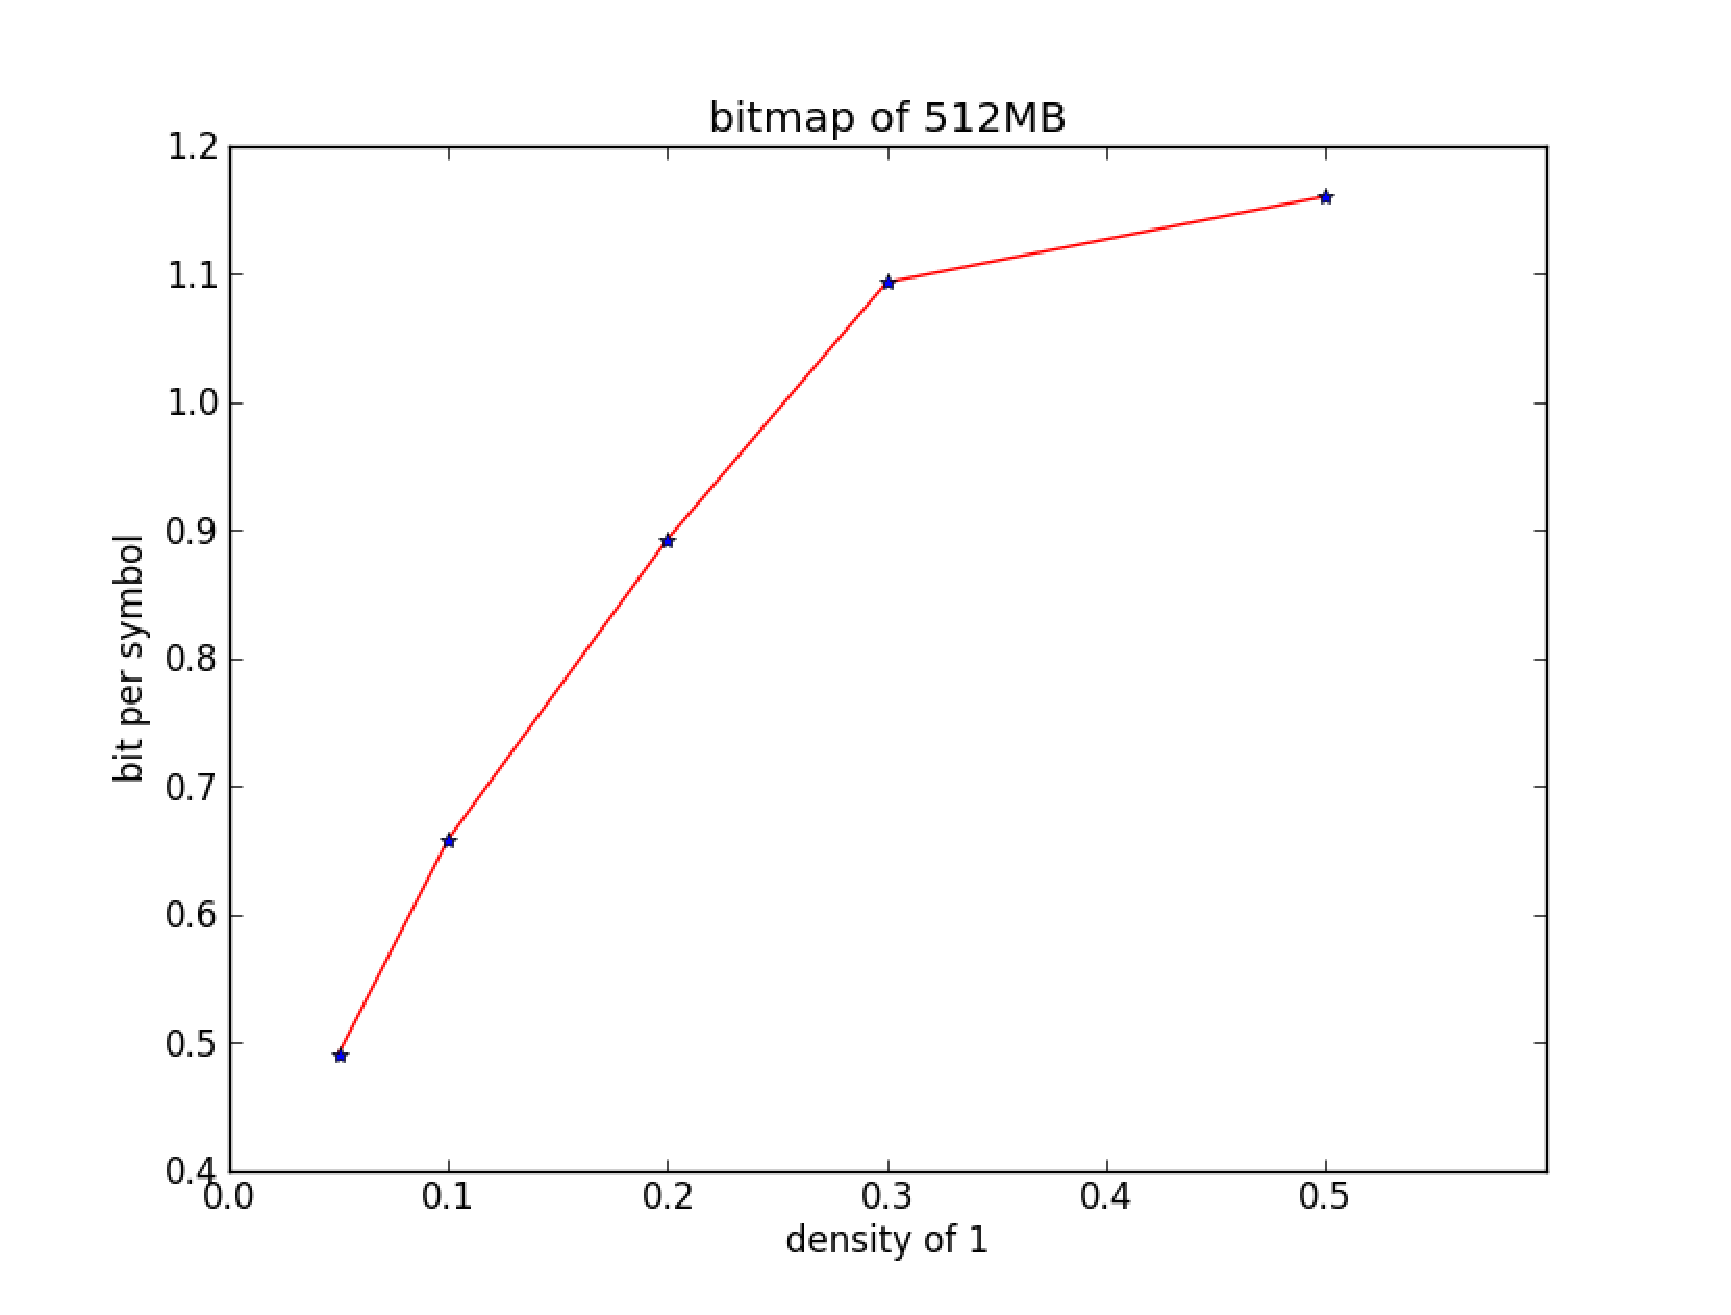
\includegraphics[width=0.8\textwidth]{rrr}
    \caption{RRR方法压缩率随序列经验熵的变化曲线}
\end{figure}


除了经典的RRR方法之外,近年来还出现了一些很有效的rank\&select数据结构实现\cite{okanohara2007practical},其中esp,recrank,vcode以及
sdarray都是类似于RRR方法,bit per symbol有可能达到小于1的实现。这些方法的性能表现在文献\cite{claude2009practical}和文
献\cite{okanohara2007practical}中都有详尽的叙述,这里只展示在空间占用上RRR方法和这几种方法的对比。

\begin{table}[htbp]
    \caption{RRR方法和其他几种方法的压缩效率对比}
    \label{tab:tabcom}
    \centering
    \begin{tabular}{lr}
    \toprule
    数据结构&Bit Per Symbol\\
    \midrule
    rrr&0.48\\
    sdarray&2.05\\
    recrank&1.25\\
    esp&0.50\\
    \bottomrule
    \end{tabular}
\end{table}

表\ref{tab:tabcom}中列出了几种方法和RRR方法的bit per symbol的大小对比,数据来源是论文\cite{claude2009practical},其测试数据是
500M的01序列,1的比例是5\%。在这一条件下,可以看到RRR方法具有明显的空间优势,其压缩率是最高的。

通过对RRR方法实现并和Jacobson的方法做实验对比,可知,在01序列并不均匀时,采用RRR方法具有明显的空间优势。而压缩后缀数组的
实现中所用得到的支持rank操作的字典则都是01序列不均匀分布的,所以在CSA中采用RRR方法实现rank操作会有更好的空间效果。Select操
作的实现是在rank的基础上实现的,总的时间复杂度可以看作rank操作的整数倍。在select操作相对于rank操作较少时,具有较好的表现。
RRR方式总体的效果是比较理想的,尤其是在空间占用上具有很大的优势,在实际应用中,若01序列的分布是很悬殊的,则RRR将是很可取的
一种rank\&select操作实现。

\section{压缩后缀数组和模式匹配}
\subsection{CSA前向搜索模式匹配算法}
从上一节对CSA性质的介绍中,我们知道后缀$T_{SA[\alpha(c)]},T_{SA[\alpha(c)+1]}\ldots T_{SA[\alpha(c)+\beta(c)-1]}$的首字符都
是$c$。设需要搜索的模式为$P[0\ldots m-1]$,首先对于字符$P[0]$,明显的其对应的在$T$中出现的位置为
$SA[\alpha(c)],SA[\alpha(c)+1]\ldots SA[\alpha(c)+\beta(c)-1]$,这个位置集可以表示为$SA[\alpha(c)\ldots\alpha(c)+\beta(c)-1]$,计为
$(l,r)$,称为后缀范围(suffix range)。下一步搜索$P[1]$,即检测$T[SA[\alpha(P[0])]+1],T[SA[\alpha(P[0])+1]+1],\cdots ,T[SA[\alpha(P[0])+\beta(P[0])-1]+1]$
是否等于$P[1]$。由后缀数组的性质可知,这一步的结果得到的后缀数组的下标依然是连续的。以此类推,直到模式串中最后一个字
符搜索完毕,即可得到匹配结果。

近一步观察上面的比较,可以发现,比较$T[SA[\alpha(P[0])]+1],T[SA[\alpha(P[0])+1]+1],\cdots ,T[SA[\alpha(P[0])+\beta(P[0])-1]+1]$
是否等于$P[1]$时并不需要比较字符串。因为$P[1]$对应的也有一个序列$SA[\alpha(P[1])],SA[\alpha(P[1])+1],\cdots ,SA[\alpha(P[1])+\beta(P[1])-1]$,所以只需要求出
$SA[\alpha(P[0])]+1,SA[\alpha(P[0])+1]+1,\cdots ,SA[\alpha(P[0])+\beta(P[0])-1]+1$和$SA[\alpha(P[1])],SA[\alpha(P[1])+1],\cdots ,SA[\alpha(P[1])+\beta(P[1])-1]$
的交集即为模式串$P[1]P[2]$出现的位置。

在上面的迭代过程中要求$SA[\alpha(P[0])]+1,SA[\alpha(P[0])+1]+1,\cdots ,SA[\alpha(P[0])+\beta(P[0])-1]+1$和$SA[\alpha(P[1])],SA[\alpha(P[1])+1],\cdots ,SA[\alpha(P[1])+\beta(P[1])-1]$的交集。
实际计算中无需求出相应的$SA$值,只需求出其对应后缀范围的交集即可,此时可以利用压缩后缀数组的性质$SA[i]+1=SA[\Phi[i]]$,
所以在计算中只需计算$\alpha(P[1]),\alpha(P[1])+1,\cdots , \alpha(P[1])+\beta(P[1])-1$和$\Phi[\alpha(P[0])],\Phi[\alpha(P[0])+1],\cdots , \Phi[\alpha(P[0])+\beta(P[0])-1]$
的交集即可。以此类推,可得到模式串$P$的后缀数组范围。

具体的算法描述如算法\ref{alg:forwardsearch}。

\begin{algorithm}
    \caption{前向搜索模式匹配}
    \label{alg:forwardsearch}
    \begin{algorithmic}[1]
        \Require $P,\Phi,\alpha,\beta$
        \Ensure $(l,r)$
        \Function{forwardSearch}{$P,\Phi,\alpha,\beta$}
        \State $m \gets size(P)$
        \State $n \gets size(CSA)$
        \State $(l,r) \gets (\alpha(P[0]),\alpha(P[0])+\beta(P[0])-1)$
        \For {$i \gets 1$ to $m-1$}
            \State $(l_{tmp},r_{tmp}) \gets (\alpha(P[i]),\alpha(P[i])+\beta(P[i])-1)$
            \For {$j \gets l$ to $r$}
            \If{$\Phi[j] \in (l_{tmp},r_{tmp})$}
                \State $l\gets j$
                \State break
            \EndIf
            \EndFor
            \For {$j \gets r$ down to $l$}
            \If{$\Phi[j] \in (l_{tmp},r_{tmp})$}
                \State $r\gets j$
                \State break
            \EndIf
            \EndFor
            \If{$l > r$}
                \State \Return $\varnothing$
            \EndIf
        \EndFor
        \State \Return $(l,r)$
        \EndFunction
    \end{algorithmic}
\end{algorithm}

算法\ref{alg:forwardsearch}的搜索过程和基于后缀数组的模式匹配算法是等价的。只是这里利用了$\Phi$数组的特性,总的时间复杂度
依然是$O(m\log n)$。

\subsection{CSA后向搜索模式匹配}
压缩后缀数组上的后向搜索模式匹配算法是由Sadakan最早提出来的\cite{sadakane2002succinct}。如上文中所述,我们用$(l,r)$
表示一个模式串在$T$上的后缀位置,模式匹配的目的正是要找到$P$的$(l,r)$。首先,计算$P[m]$的后缀位置,很明显$(\alpha(P[m]),
\alpha(P[m])+\beta(P[m])-1)$就是。假设一般情况,我们已经知道$P[i+1\ldots m-1]$的后缀数组位置为$(l_{P_{i+1}},r_{P_{i+1}})$,
那么$P[i\ldots,m-1]$的后缀数组位置$(l_{P_i},r_{P_i})$必定是由$P[i]$的后缀数组位置的一部分组成的,设$P[i]$的后缀数组位置
为$(l_{P[i]},r_{P_i})$,那么对于$l_{P[i]\leq k \leq r_{P_i}}$只要$SA^{-1}SA[k]+1$在$(l_{P_{i+1}},r_{P_{i+1}})$中,$k$一定在$(l_{P_i},r_{P_i})$
中。也就是说$P[i\ldots n-1]$的出现位置一定是$P[i]$的出现位置后面紧跟着$P[i+1\ldots m-1]$的出现位置。加上$\Phi[i]=SA^{-1}[SA[i]+1]$,
所以我们可以得到公式\ref{equa:equa1}。

\begin{equation}\label{equa:equa1}
    k \in (l_{P_i},r_{P_i}) \iff k \in (l_{P[i]},r_{P[i]}) \wedge \Phi[k] \in (l_{P_{i+1}},r_{P_{i+1}})
\end{equation}

由于在简明数据结构存储下$\Phi$可以在常数时间内获得,并且其值在$(l_{P_{i+1}},r_{P_{i+1}})$上是递增的,所以,可以用二分搜索
来搜索$\Phi[k]$是否在$(l_{P_{i+1}},r_{P_{i+1}})$上,时间复杂度是$O(\log n)$。重复上述过程$m$次,即可在CSA上用$O(m\log n)$
时间复杂度找到模式$P[0\ldots m-1]$的后缀数组范围$(l,r)$

算法\ref{alg:backwardsearch}给出了CSA上的后向搜索的伪代码。而图\ref{figbackwardsearch}给出了一个采用算法\ref{alg:backwardsearch}
的例子,搜索模式$P=CCAGTA$。每一个方块儿对应一个字符的后缀数组区域,灰色的区域表示对应$P$的一个后缀在$T$的后缀数组上的位置
范围。在右起第二步,计算新的区域时,根据下一个字符$G$的后缀范围,计算其$\Phi$值,查看这个$\Phi$是否落在当前模式$TA$的后缀范
围内,由于$\Phi$的递增特性,很容易用二分搜索方法找到新的区域的上下界。

\begin{algorithm}
    \caption{后向搜索}
    \label{alg:backwardsearch}
    \begin{algorithmic}[1]
        \Require $P,\Phi,\alpha,\beta$
        \Ensure $(l,r)$
        \Function{backwardSearch}{$P,\Phi,\alpha,\beta$}
        \State $l_{m} \gets 0;r_{m}\gets n-1$
        \For {$i\gets m-1$ down to $0$}
            \State $l_i \gets \min\{ k \in [\alpha(P[i]),\alpha(P[i])+\beta(P[i])-1],\Phi[k] \in [l_{i+1},r_{i+1}]\}$
            \State $r_i \gets \max\{ k \in [\alpha(P[i]),\alpha(P[i])+\beta(P[i])-1],\Phi[k] \in [l_{i+1},r_{i+1}]\}$
            \If{$l> r$}
                \State \Return $\varnothing$
            \EndIf
        \EndFor
        \State \Return $(l_0,r_0)$
        \EndFunction
    \end{algorithmic}
\end{algorithm}


\begin{figure}[t]
    \centering
    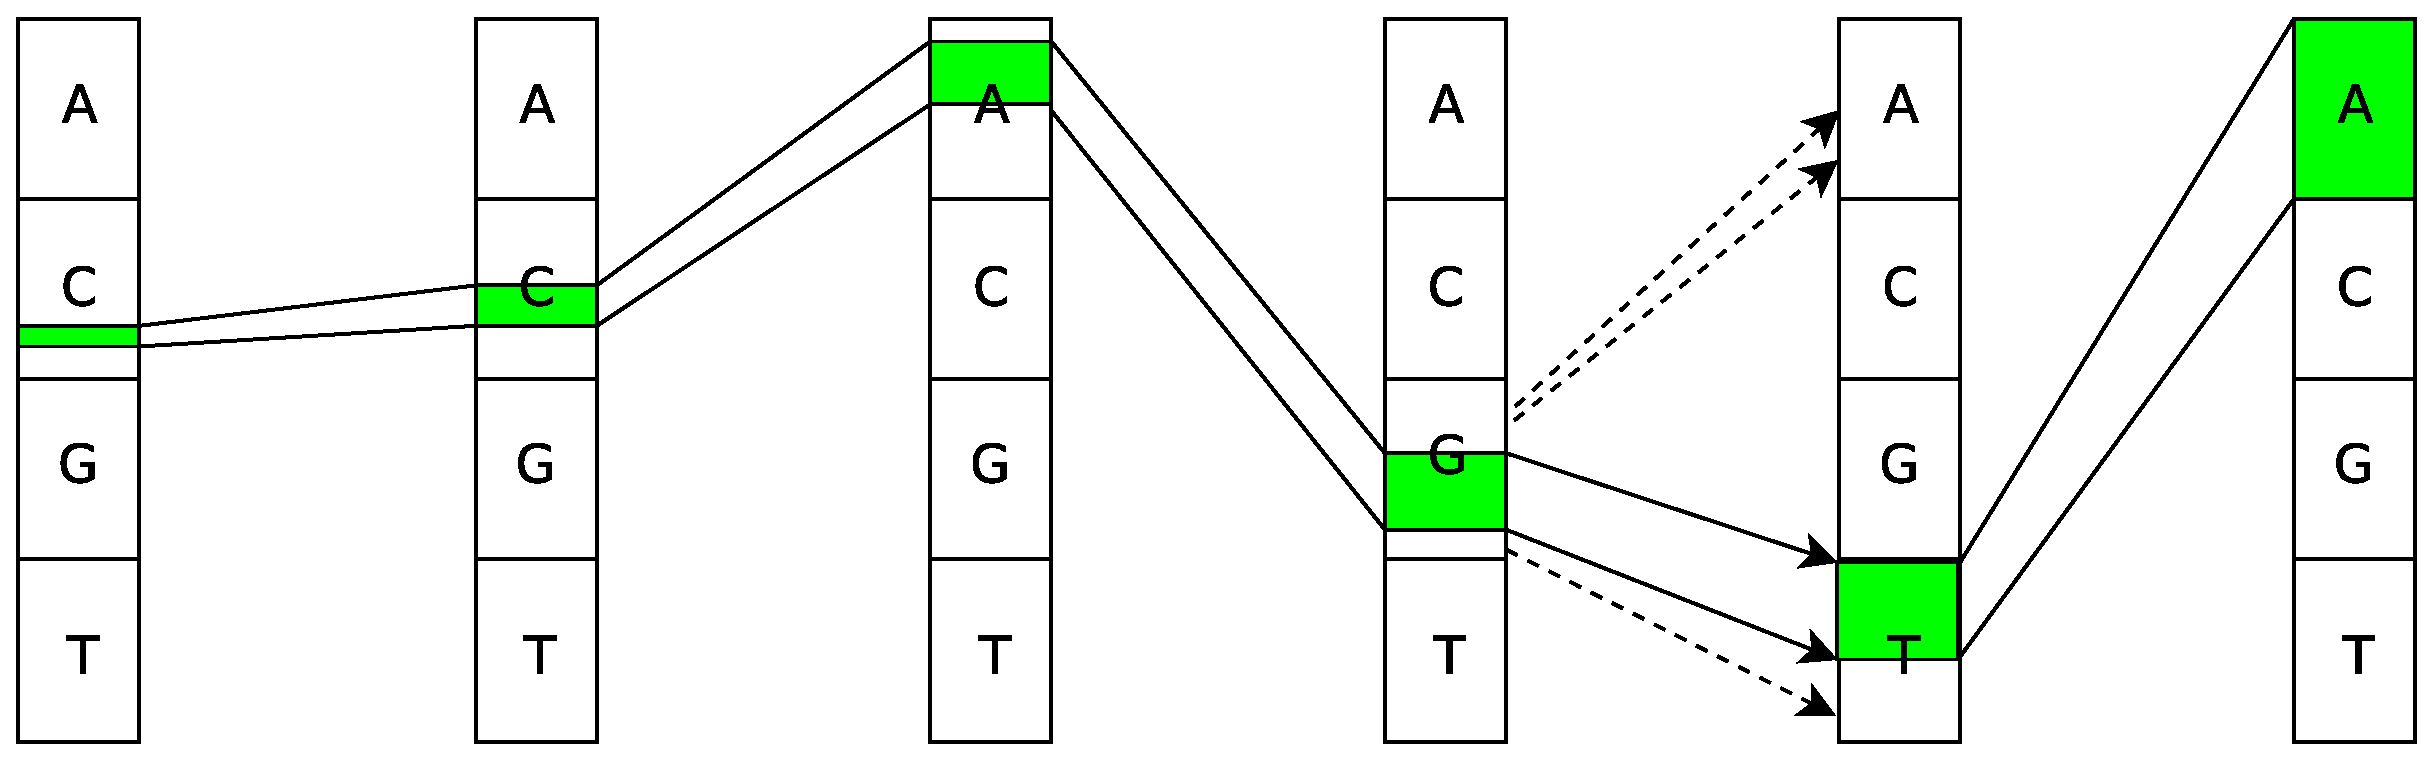
\includegraphics[width=0.7\textwidth]{csa_backwardsearch}
    \caption{CSA上的后向搜索}
    \label{figbackwardsearch}
\end{figure}

\section{压缩后缀数组和自索引}
压缩后缀数组优于后缀数组的另一性质是其自索引性。在上一小节的模式匹配算法中,可以看到并不需要原文本$T$即可完成匹配,
基于这个原理,只要给压缩后缀数组添加一个辅助数组即可实现压缩后缀数组的自索引算法。

考虑已知$\Sigma$中任意字符$c$的$\alpha(c)$值,则$\beta(c)=\alpha(c+1)-\alpha(c)$,所以只需保存$\alpha(c)$即可完成
无需原文本的模式匹配,基于此在压缩后缀数组基础上增加一个辅助数组$\alpha$即可实现自索引。

考虑下面的性质$T[SA[\alpha(c)]]=T[SA[\alpha(c)+1]]=\cdots=T[SA[\alpha(c)+\beta(c)-1]]=c$,所以对于$T$中任意位置$i$处
的字符,只要求出其对应后缀$T_i$的名次,即$j=SA^{-1}[i]$,便可在$\alpha$数组中搜索其所在区间使得对某个字符$c$存
在$\alpha(c)\leq j< \alpha(c+1)$,即得到$T[SA[j]]=c$,所以即可知$T[i]=c$。而由前文中可所述$\Phi$的性质可知后缀数组的
逆数组$SA^{-1}$是可以在线性时间内得到的。

按照上面叙述的方法可以很方便的恢复出文本$T$的任意字符,进而恢复出$T$的任意长的子串$T_{i,j}$。在实际运算中
考虑到压缩后缀数组的性质$SA^{-1}[i+1]=\Phi[SA^{-1}[i]]$,所以在已知$SA_[i]$求出$T[i]$的情况下求$T[i+1]$时,
不必再求$SA^{-1}[i+1]$,直接返回$\Phi[SA^{-1}[i]]$,这个计算是常数时间的,而不是线性时间\cite{sadakane2000compressed}。

具体算法如算法\ref{alg:getT}。

\begin{algorithm}[ht]
    \caption{CSA自索引}
    \label{alg:getT}
    \begin{algorithmic}[1]
        \Require $\Phi,\alpha,i,j$
        \Ensure $T[i\ldots j]$
        \For {$k\gets i$ to $j$}
            \If {k=i}
                \State $rank \gets SA^{-1}[k]$
                \State $prev \gets rank$
            \Else
                \State $rank \gets \Phi[prev]$
            \EndIf
            \State $T[k] \gets$ \Call{binarySearch}{$rank$,$\alpha$}
        \EndFor
        \State \Return $T[i\ldots j]$
    \end{algorithmic}
\end{algorithm}

上述算法总共执行$m=j-i+1$步,每一步执行一次$|\Sigma|$上的二分搜索,且要求$SA$,所以时间复杂度为
$O(\log |\Sigma|+\log \log n)$,所以总的时间复杂度为$O(m(\log |\Sigma|+\log \log n))$。

\section{本章小结}
本章主要在前面阐述的后缀数组和压缩后缀数组性质的基础上提出了基于压缩后缀数组的文本索引和自索引算法。并详细介绍了上实现压缩
后缀数组的基本数据结构:RRR算法。之后介绍了两种CSA上的$O(m\log n)$时间复杂度的模式匹配算法:前向搜索和后向搜索。为下一章的
DNA序列比对算法给出实现基础。最后还介绍了CSA的自索引性质,并给了由压缩后缀数组恢复原文本序列的算法。

    \chapter{基于压缩后缀数组的序列比对算法}
本章将介绍基于CSA的短读比对算法(CSAA)。CSAA采用CSA索引参考序列,利用CSA的后向搜索完成匹配过程。CSA的后向搜索是一种精确匹配
算法,可以在$O(m\log n)$是间复杂度内找出长为$m$的模式$P$在长为$n$的序列中的后缀数组位置。然而,由于DNA序列存在个体变异,以及测
序技术有一定的错误率,反应在短读序列上就是短读序列的每一个核苷酸并非都是可靠的,所以在做短读映射时就不能简单的使用精确模式匹配
算法,而应该尽可能根据短读序列的性质找到一个最可靠的匹配位置。本文提出了两种策略来实现短读比对中的非精确匹配
要求。一是在后向搜索过程中引入了搜索树,使得在短读匹配过程中可以随时对短读序列上的某个核苷酸进行插入,删除,替换等操作,达到模
糊匹配的目的。另一个策略是在搜索树上引入优先堆的数据结构,这一数据结构结合评分机制保证在后向搜索的每一步中都是沿着最优的搜索
方向前进,并且采用分支限界的策略适时淘汰很差的搜索方向,最终实现找到一个最优的匹配位置的目的。

\section{精确匹配}
精确匹配本质上就是是后向搜索。根据算法\ref{alg:backwardsearch},可知给定一个长为$n$的参考序列$T$,$P$为测序得到的短读序列中的
一个短读,假设已经获取到短读的后缀$P[i+1\ldots m-1]$的后缀数组位置$(l_{P_{i+1}},r_{P_{i+1}})$,那么可以跟据公式\ref{equa:exac}
确定后缀$P[i\ldots m-1]$的后缀数组位置$(l_{P_i},r_{P_i})$。

\begin{equation}\label{equa:exac}
    \begin{split}
        l_{P_i} \gets &\min\{ k \in [\alpha(P[i]),\alpha(P[i])+\beta(P[i])-1],\Phi[k] \in [l_{P_{i+1}},r_{P_{i+1}]}\}\\
        r_{P_i} \gets &\max\{ k \in [\alpha(P[i]),\alpha(P[i])+\beta(P[i])-1],\Phi[k] \in [l_{P_{i+1}},r_{P_{i+1}]}\}
    \end{split}
\end{equation}

由于$\Phi[\alpha(P[i])\ldots \alpha(P[i])+\beta(P[i])-1]$是严格递增序列,所以公式\ref{equa:exac}可以采用二分搜索实现。
搜索$[\alpha(P[i],\alpha(P[i])+\beta(P[i])-1]$的
左边界和右边界在$\Phi[\alpha(P[i])\ldots \alpha(P[i])+\beta(P[i])-1]$上是否出现,即可得$P[i\ldots n-1]$的后缀数组
位置$(l_{P_i},r_{P_i})$。

综上所述,可以得到以下精确匹配算法\ref{alg:exac},该算法采用后向搜索的方法,根据一个给定的模式$X$的后缀数组$(l,r)$和
字符$c$计算出新模式$cX$的后缀数组位置。根据这个算法,加上一定策略,即可得到我们下文将提出的近似匹配算法。

\begin{algorithm}
    \caption{精确匹配}
    \label{alg:exac}
    \begin{algorithmic}[1]
        \Require $\Phi,\alpha,\beta,l_{old},r_{old},c$
        \Ensure $(l,r)$
        \Function{ExactMatch}{$\Phi,\alpha,\beta,l_{old},r_{old},c$}
        \State $l_c \gets \alpha(c)$
        \State $r_c \gets \alpha(c)+\beta(c)-1$
        \State $(l,r) \gets $\Call{binarySearch}{$\Phi[l_c\ldots r_c],l_{old},r_{old}$}
        \If{$l>r$}
            \State \Return $\varnothing$
        \Else
            \State \Return $(l,r)$
        \EndIf
        \EndFunction
    \end{algorithmic}
\end{algorithm}

\section{近似匹配}

根据上一小节所述的精确匹配算法思想,模式匹配就只有两种结果,要么匹配上,要么没匹配上这种完全的匹配方式并不适合大多数存在变异
和测序误差的短读序列。本文提出的CSAA算法是建立在非精确匹配的基础上的。

由于同一物种之间存在的个体差异(具体在DNA上表现为单核苷酸变异SNP),以及测序技术存在的误差,Resequencing技术得到的短读序列和
该物种的标准参考序列之间哪怕是同一基因片段也必然存在着一些不同,这会造成即使同一种基因序列也无法完全比对映射到参考序列上。
所以对短读和参考序列之间的比对仅仅精确比对映射是远远不够的,这会造成大量的短读因为和参考序列相差一两个核苷酸不同而不能映射
到参考序列上,而这一两个不同的核苷酸很可能是测序误差或者生物个体之间的SNP造成的,不应当认为二者是不能匹配的。所以,采用合适
的非精确比对算法是必须的。本文提出的非精确匹配算法中,支持对短读进行替换(substitude),插入(insert),删除(delete)三种变换操
作,通过这三种操作可以保证变异的或者发生测序错误的短读序列依然能正确匹配到参考序列的合适位置上。

考虑一个给定的长为$m$的短读序列$P$,采用后向搜索,当搜索到第$i+1$个位置时,得到序列$P_{i+1}$的后缀数组位置$(l_{i+1},r_{i+1})$,
依照精确匹配的算法下一步应当在$(l_{i+1},r_{i+1})$的基础上搜索字符$P[i]$,从而得到一个新的后缀数组位置$(l_i,r_i)$。在此,如果我们不
搜索$P[i]$,而是搜索另一个符号$c \neq P[i]$,得到另一个后缀数组位置$(l_{i}^{'},r_{i}^{'})$。接着在$(l_{i}^{'},r_{i}^{'})$基础
上继续搜索$P[0\ldots i-1]$,那么最终得到后缀数组位置$(l_0,r_0)$将不再是序列$P$的一个后缀数组位置了,而是将$P[i]$替换为$c$
后的新字符串的后缀数组位置。称这个新位置为$P$的一个替换近似串的后缀数组位置,计为$(l_0,r_0,m,P(S_i))$,即长为$m$的序列$P$在
$i$位置进行一次替换后可以映射到参考序列的后缀数组位置$(l_0,r_0)$。

图\ref{fig:substitude}给出了把短读序列中的一个符号$T$替换为$A$时的搜索过程,实线为精确匹配的过程,虚线是替换后的搜索过程。

\begin{figure}[htbp]
    \centering
    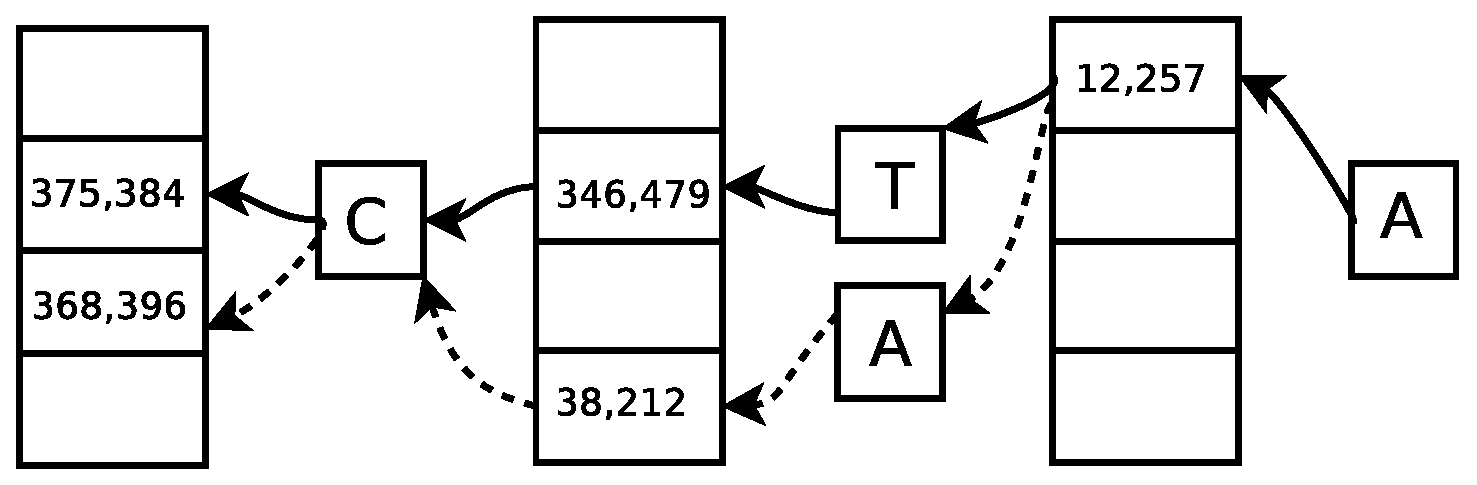
\includegraphics[width=0.7\textwidth]{substitude.eps}
    \caption{替换操作示例} \label{fig:substitude}
\end{figure}

不同于替换操作,如果在搜索到$P[i]$时,放弃搜索$P[i]$符号,直接在$(l_{i+1},r_{i+1})$的基础上搜索序列$P[0\ldots i-1]$,那么
最终得到的后缀数组位置$(l_0,r_0)$将是$P$删除$P[i]$后的近似串在参考序列上的后缀数组位置,计为$(l_0,r_0,m,P(D_i))$,,即长为$m$
的序列$P$在$i$位置进行一次删除后可以映射到参考序列的后缀数组位置$(l_0,r_0)$。

如图\ref{fig:delete}所示为删除短读序列中的一个符号后的搜索过程。

\begin{figure}[htbp]
    \centering
    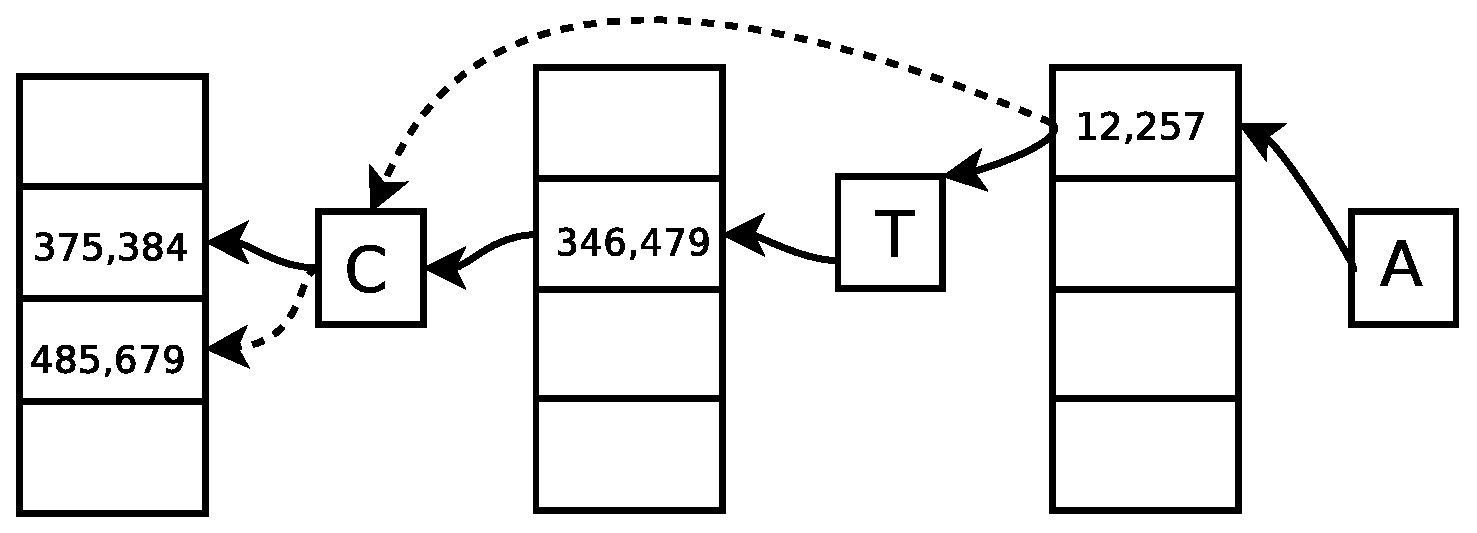
\includegraphics[width=0.7\textwidth]{delete.eps}
    \caption{删除操作示例} \label{fig:delete}
\end{figure}

对于插入操作,在搜索到$P[i]$时,不直接搜索$P[i]$,而是在$l_{i-1},r_{i-1}$的基础上搜索符号$c$,得到$(l_{i}^{'},r_{i}^{'})$,接着
在此基础上搜索序列$P[0\ldots i]$,最终得到的后缀数组位置$(l_0,r_0)$将是$P$在$i$位置插入符号$c$后的近似序列的后缀数组位置。计为
$(l_0,r_0,m,P(Ii)$,即长为$m$的序列$P$在$i$位置插入一个符号后可以映射到参考序列的后缀数组位置$(l_0,r_0)$。

如图\ref{fig:insert}所示为插入一个符号'A'前后的短读序列中的一个符号后的搜索过程。

\begin{figure}[htbp]
    \centering
    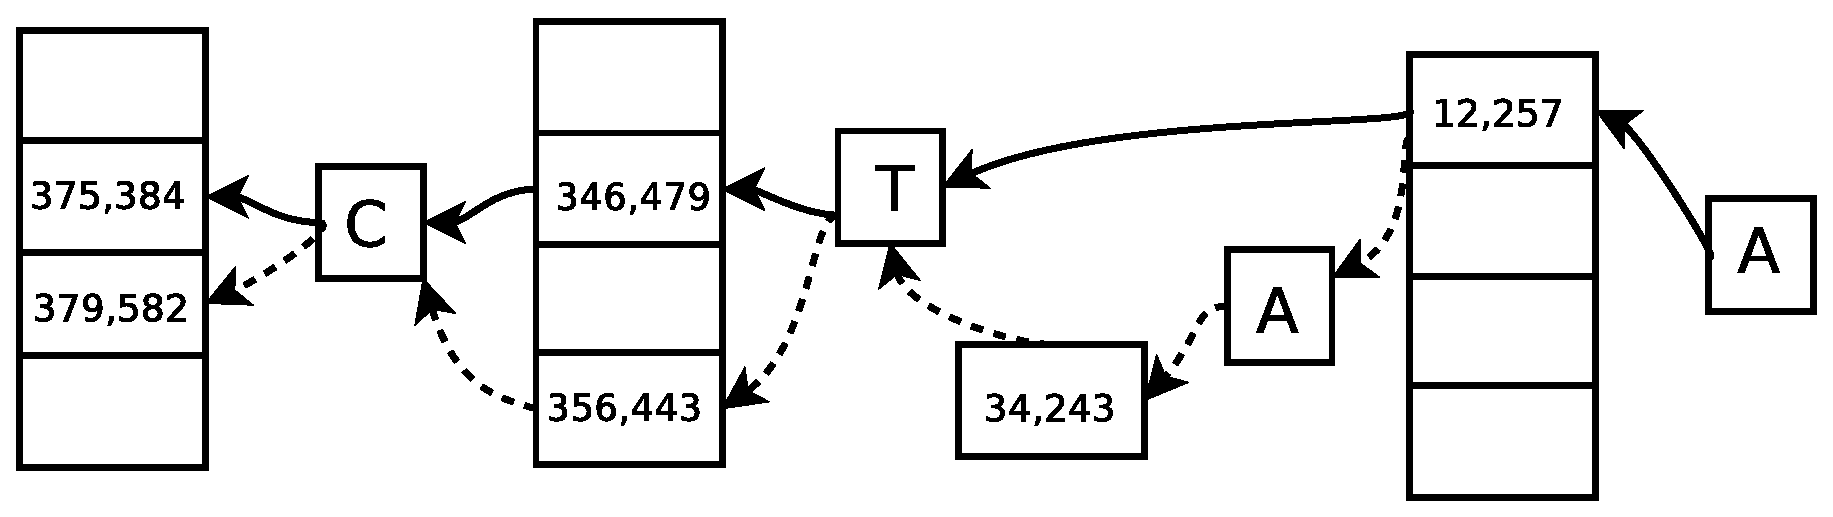
\includegraphics[width=0.7\textwidth]{insert.eps}
    \caption{插入操作示例} \label{fig:insert}
\end{figure}

综上所述,通过在搜索的过程中加入替换,删除,插入三种操作,可以扩展后向搜索的搜索方向,达到近似匹配的目的。如果已知模式串的
某个字符是不可靠的,那么我们可以通过在这个位置加入上述三种操作,实现非精确匹配,查找到这个模式串的可能匹配位置。而大多数情况
下,我们是不知道具体哪一个字符不可靠的,所以只能试探每一个字符,对每一个字符都做删除,替换,插入操作,从而找到一个合适的位置。
据此,我们提出非精确匹配算法\ref{alg:inexact},这个算法递归的实现近似匹配,对$P$的每一个位置都做了三种操作,所以这个算法的本
质是对长为$m$的序列$m$做了所有可能的近似串的搜索,即做了$|\Sigma|^m$个序列的匹配。因为采用了后向搜索的过程,每一次递归实际都
是产生$\Sigma$次替换递归,$\Sigma$次插入递归,和1次删除递归,所以实际的时间复杂度
满足递归式\ref{equa:exact}。解递归式\ref{equa:exact}可得$T(m)=(2\Sigma+1)^{m-1}+\Theta(m\log n)$。
\begin{equation}\label{equa:exact}
    T(m)=\begin{cases}\Theta(1) & \mbox{if } m=1 \\
    2(\Sigma+1)T(m-1)+\Theta(\log n) & \mbox{if } m>1\end{cases}
\end{equation}

\begin{algorithm}
    \caption{近似匹配}
    \label{alg:inexact}
    \begin{algorithmic}[1]
    \Require $\Phi,\alpha,\beta,l,r,P,i$
    \Ensure $(l,r)$
    \Function{inexactMatch}{$\Phi,\alpha,\beta,l,r,P,i$}
    \If{$i<0$}
    \State \Return $(l,r)$
    \EndIf
    \State $S \gets \varnothing$
    \State $S \gets S\ \cup$\ \Call{inexactMatch}{$\Phi,\alpha,\beta,l,r,P,i-1$} \Comment{删除$P[i]$操作}
    \ForAll{$c \in \Sigma$}
    \State $(l,r)\gets$\Call{ExacMatch}{$\Phi,\alpha,\beta,l,r,c$} \Comment{调用算法\ref{alg:exac}}
        \If{$l\leq r$}
        \State $S \gets S\ \cup\ $ \Call{inexactMatch}{$\Phi,\alpha,\beta,l,r,P,i-1$} \Comment{替换$P[i]$为$c$}
        \State $S \gets S\ \cup\ $ \Call{inexactMatch}{$\Phi,\alpha,\beta,l,r,P,i$} \Comment{在$P[i]$后插入$c$}
        \EndIf
    \EndFor
    \State \Return $S$
    \EndFunction
\end{algorithmic}
\end{algorithm}

\section{搜索树}

根据上一小节中描述的方法,用后向搜索实现替换,删除,插入操作的方法,实现短读序列的近似匹配。在不知道具体的替换,删除以及插入
位置时,需要在每一次后向搜索一个符号时都分别做一次替换,删除,插入操作。而每一次操作实际上都导致了一个新的近似序列的产生,在
未完成整个序列的搜索时,最终哪一个近似序列能够较好的映射到参考序列上依然是未知的,这就要求我们在搜索过程中保留每一个可能的近
似序列。

\begin{figure}[htbp]
    \centering
    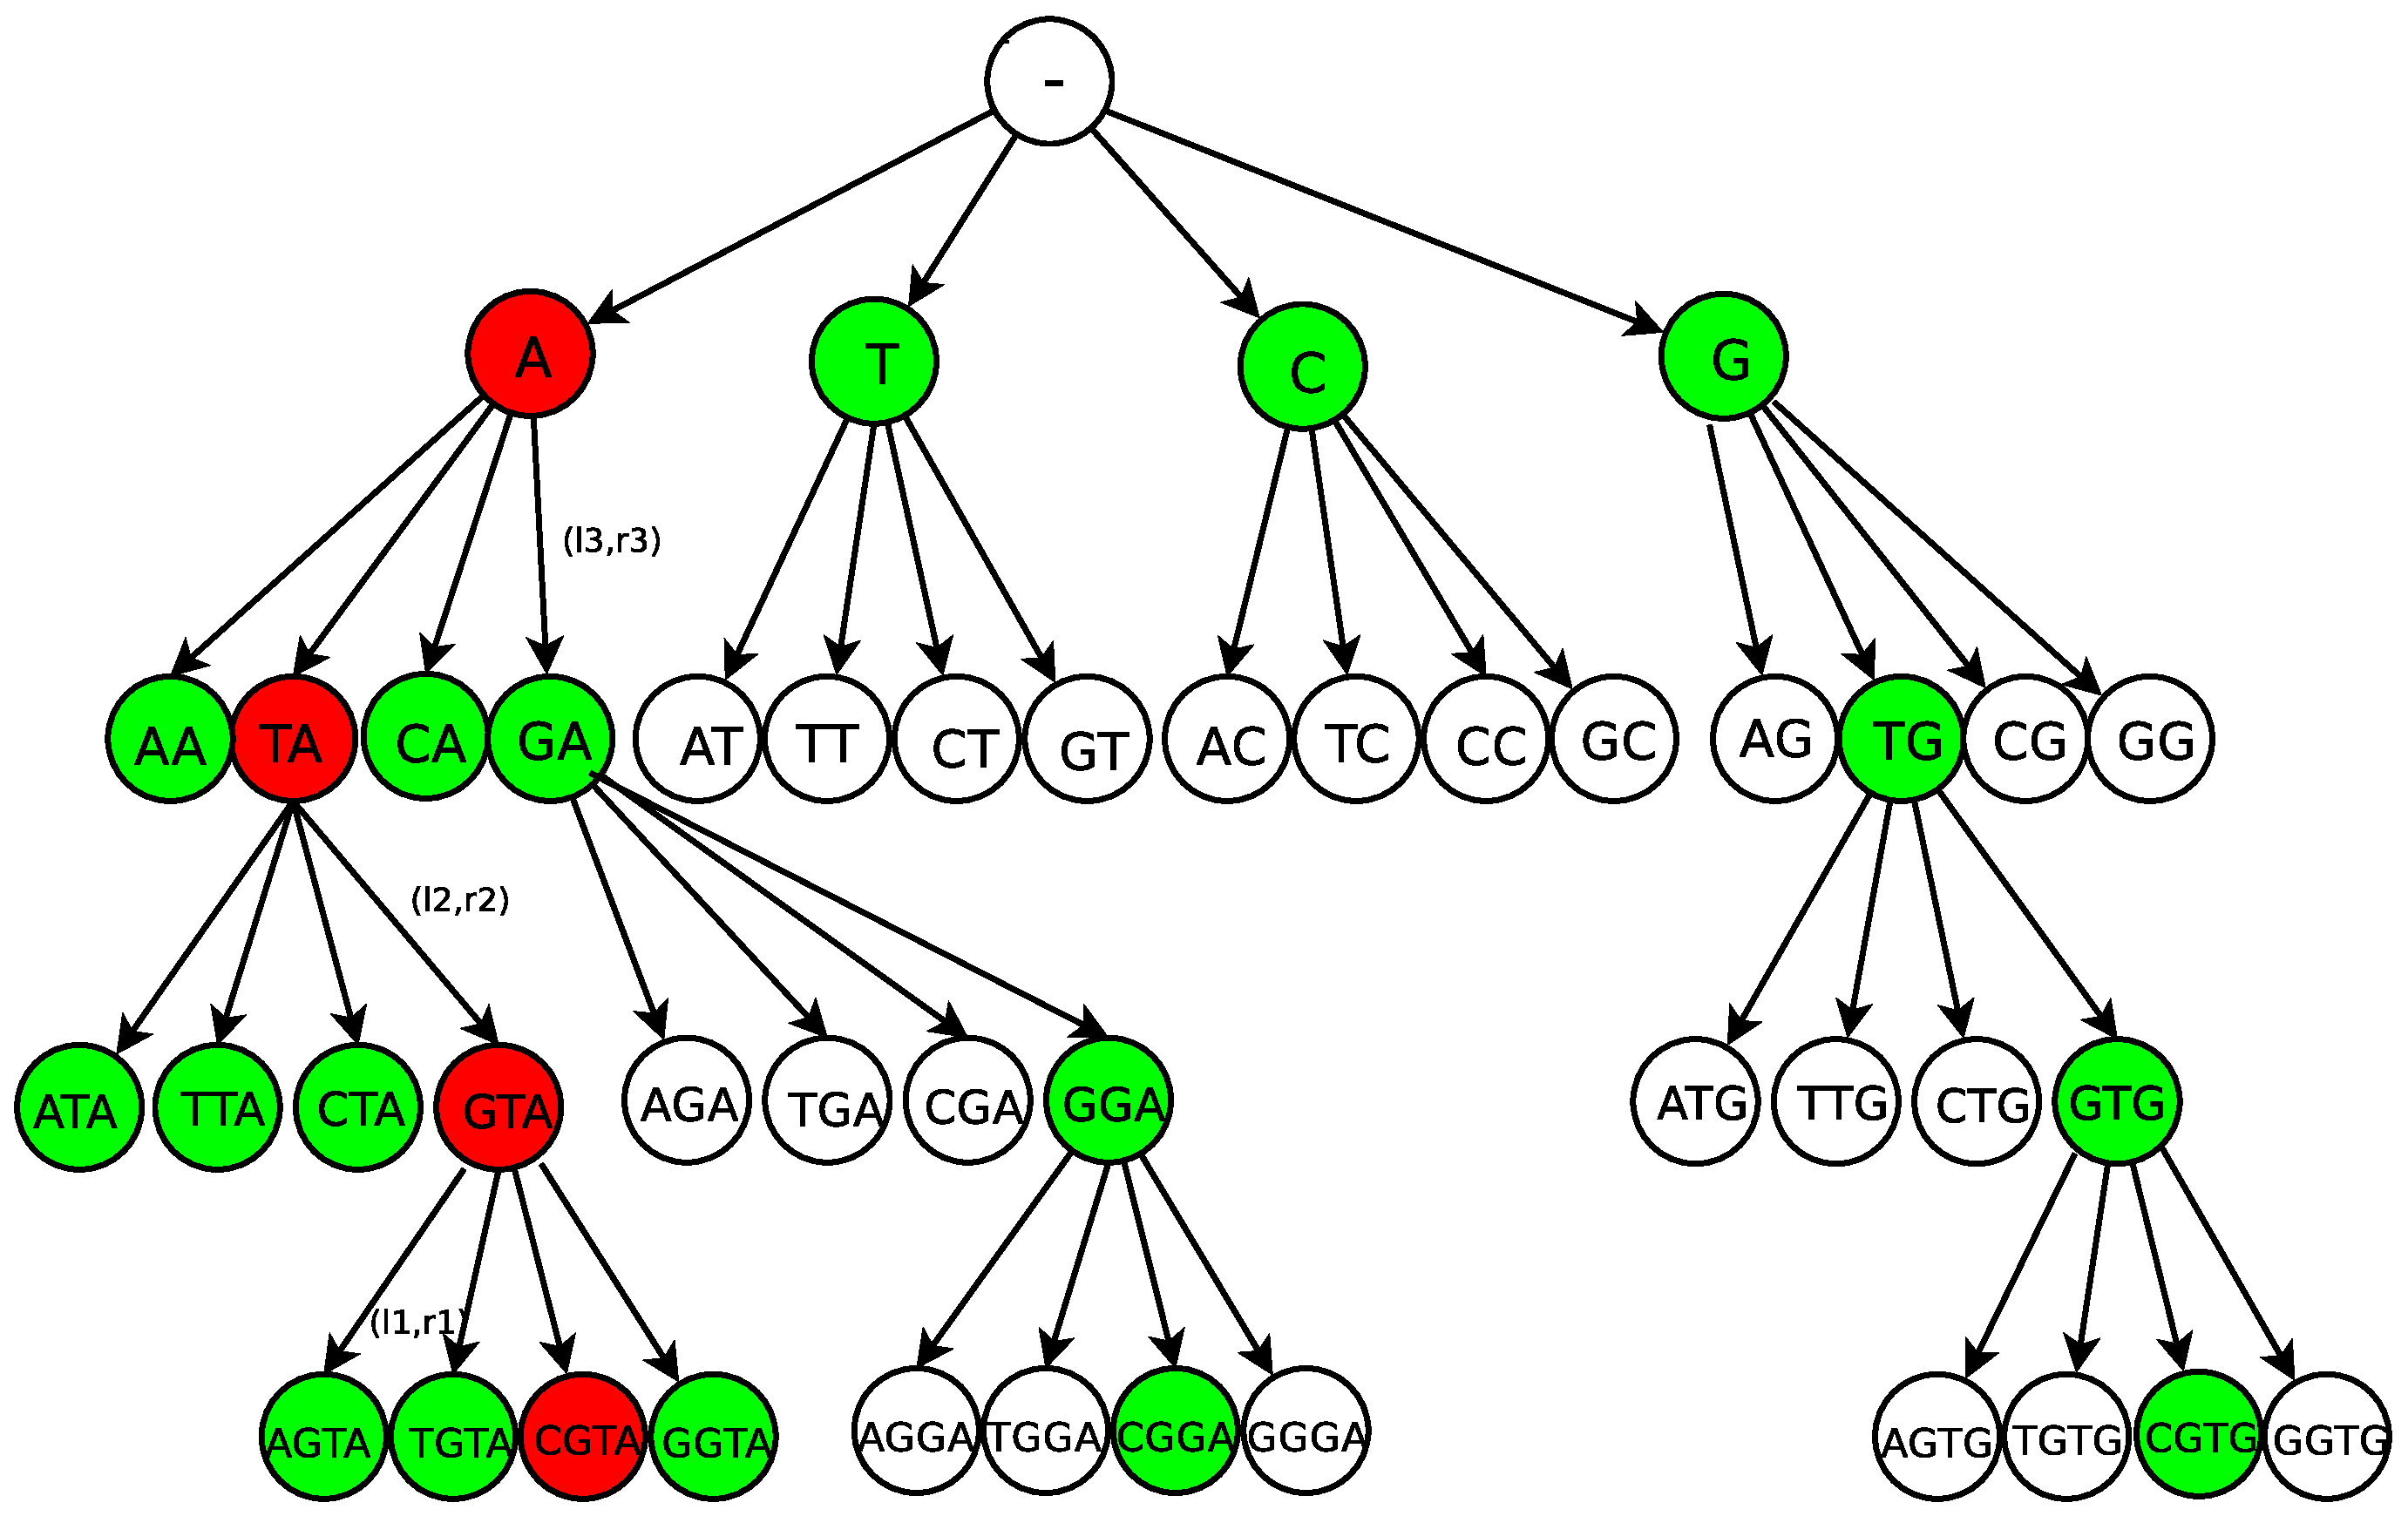
\includegraphics[width=0.9\textwidth]{searchtree.eps}
    \caption{近似匹配示例} \label{fig:searchtree}
\end{figure}

实际上,每一次的替换,删除或者插入操作导致的新的近似序列可以看作一个树上的遍历过程。如图\ref{fig:searchtree}所示,对于一个长
为4的短读 $P=$``CGTA''的搜索过程,简化起见,省略了删除和插入操作。首先通过CSA查询$P[3]=$`A'在参考序列上的后缀数组位置。接着把
$P[3]=$`A'分别替换为`T',`C',`G',在CSA上查找替换后的后缀数组位置。图中红色路径标志的是到当前搜索深度没有替换操作的近似串,而
绿色标记的则是到当前深度有一次替换操作的近似串,无色的是有两次以上替换操作的近似串搜索路径。可以看到,随着搜索深度的增加,搜索
的方向急剧扩大,加上还有未画出的删除和插入操作,可能的搜索方向会更多。

搜索树的本质是对每一个可能的近似序列都进行搜索,假设一个短读序列的长度为$m$,DNA序列字符集为4,根据上一小节,总的时间复杂度为$9^{m-1}+\Theta(m\log n)$。
考虑到$m$一般在20到70之间,如果直接采用搜索树来进行近似匹配,搜索规模会非常大而难以在有效时间内实现。实际上也无需比对所有的近
似串,对于某些替换,删除或者插入操作过多的近似串,应该提前抛弃掉,即采用分支限界法来对搜索树进行剪枝,去除掉无效的搜索方向,降
低搜索空间。

\section{分支限界}

根据上一小节的分析,搜索树的搜索空间复杂度是随短读序列长度指数级增长的,因此必须进行适当的剪枝,抛弃一些没有价值的搜索方向。
传统的DNA序列比对中用到了编辑距离(Edit Distance),汉明距离(Hamming Distance)等来度量两个序列的相似度。在此我们也可以使用类
似的方法做分支限界,比如采用编辑距离,可通过给定一个允许的最大编辑距离$maxDistance$,当在短读序列$P$上后向搜索进行到第$i$步
时,在某个搜索方向上的一个近似序列为$P^{'}$,计算$P$和$P^{'}$之间的编辑距离,若距离大于预先定义的$maxDistance$,则抛弃这个搜
索方向,否则,保持这个搜索方向。汉明距离做分支限界的方法和编辑距离方法类似。

采用编辑距离和汉明距离的方法必须对每一个得到的近似序列和短读序列计算距离,这一方面会导致算法效率的降低,另一方面由于我们在做
短读比对时,会有大量的短读需要比对,这些短读的长度不一定都相同,指定唯一的$maxDistance$是不合适的。对此,在论文\cite{li2009fast}
中,作者提出了一种类似于编辑距离的算法,称之为$difference$数组,该算法很好的实现了自适应的类编辑距离的最大限制距离。因此本文
提出的CSAA比对算法也使用$difference$数组作为分支限界的一个条件。$difference$数组是利用$CSA$上的精确匹配算法,首先对需要比对的
短读做预处理,处理过程如算法\ref{alg:darray}所示。处理过的$difference[i]$反映了在搜索$P[i\ldots n-1]$时可以允许的最大替换,插
入,删除操作的次数。由于在序列比对中我们采用的是后向搜索的过程,所以在计算$difference$数组时,也需要从后往前算,使得$difference$
是一个递减的序列,也即在从后往前比对短读$P[0\ldots n-1]$时,越往前,允许的替换,插入,删除数量越多。

\begin{algorithm}
    \caption{计算$difference$数组}
    \label{alg:darray}
    \begin{algorithmic}[1]
        \Require $\Phi,\alpha,\beta,P$
        \Ensure $difference[0\ldots |P|-1]$
        \Function{CalculateDifference}{$\Phi,\alpha,\beta,P$}
            \State $z \gets 0$
            \State $l \gets 0$
            \State $r \gets |P|-1$
            \For{$i \gets |P|-1$ downto $0$}
                \State $(l,r) \gets$ \Call{ExactMatch}{$\Phi,\alpha,\beta,l,r,P[i]$} \Comment{调用算法\ref{alg:exac}}
                \If {$l>r$}
                \Comment{失配,$difference[i]$增加一次,否则$difference[i]$不变}
                \State $l\gets 0$
                \State $r \gets |P|-1$
                \State $z \gets z+1$
                \EndIf
                \State $difference[i] \gets z$
            \EndFor
        \EndFunction
    \end{algorithmic}
\end{algorithm}

$difference$数组的作用,是结合每一个近似序列的一个辅助值$z$来分支限界的。开始比对时,序列$P$的$z$值是$0$,之后每做一次插入,
删除或者替换,则$z$增加一次,而在该操作位置的最大允许删除,插入,替换操作数是$difference[i]$。比较两者,若$z>difference[i]$
则证明该搜索方向做了过多的替换,删除,插入操作,短读已经和参考序列相似度太小,应当删除该搜索方向,考虑搜索树上的其他方向。

除了$difference$距离,另一可用的分支限界策略是罚分机制。在搜索树上向前搜索时,每一次替换,删除或者插入操作都会产生一个新的近
似序列,而每增加一次这样的操作,都会导致这个方向上的近似序列和参考序列的相似度下降。基于此,我们可以预定义一个罚分上限$maxPenalty$。
同时为替换,插入,删除三种操作分别定义各自的罚分,当这个短读比对过程中每做一次上述操作时,都会对这个近似序列增加相应的罚分,
当罚分达到预定义的最大罚分$maxPenalty$时,即认为这个近似序列已经和短读序列相似度太小,没有必要再继续搜索这个方向。通过这样的
罚分机制,可以去除较差的近似序列,达到分支限界的目的。

在生物信息学领域,每一个删除或者插入统称为一个indel,而每一个indel都会在短读序列上造成一个空位(gap),对应的罚分称为空位罚分。
gap通常分为两种,一种是单独出现在序列中,称为gap open;另一种是连续的gap,称为gap extension。gap open的罚分是各个gap罚分的线
性叠加和,而通常gap extension的罚分不能简单的做线性增加来处理。Affine gap penalties是生物信息学领域常用的一种罚分机制,假设
有一个gap extension长为$x$,则这个gap的罚分为$-(\rho +\sigma x)$,其中$\rho >0$,$\sigma$是每一个indel操作的罚分。

有了$difference$距离和$gap$罚分两种分支限界的策略,可以大大减少搜索的规模,通过控制合适的$maxPenalty$可以实现在比对时间和比对
精度之间的平衡。然而如果直接依赖算法\ref{alg:inexact}实现比对算法也是不合适的。因为算法\ref{alg:inexact}是一个递归的算法,递
归算法本身在实际实现时过于低效,我们的short read一般都长30bp以上,这样的深度是不能用递归的。另一方面,递归比对的本质在
搜索树上表现为一个深度优先的搜索,每一次递归都会把一个方向上的所有方向做一次尝试,直到遇到分支限界条件不合适才会回溯到上一层。
这一特性会引起过度回溯的问题。这一问题的本质是每次进入一个新的搜索方向时没有做出正确的选择,整体的搜索方向是随机的,算法大多
数的递归选择都会进入不是最好的方向,从而最终不得不回溯,这显著增大了时间开销。据此本文提出一种优先堆结构,把搜索树上的深度优
先搜索改为广度优先搜索。每一层上都把所有的搜索方向排序放在一个优先堆里,算法每进入下一个搜索方向都在当前优先堆中选择最优的即
罚分最低的搜索方向进入。借助这一优先堆结构,可以把搜索方向限制在只沿着最优的搜索方向前进,从而实现最优比对。同时,还可以限定
优先堆的大小,抛弃掉虽然符合分支限界条件但相对于其他搜索方向过差的搜索方向。

优先队列使用了最大堆来实现,每一项保存一个近似匹配的序列相关匹配信息,以每个近似序列的罚分和$z$值作为优先堆的$key$值。本文中
使用的优先堆支持如下操作:

\begin{itemize}
    \item INIT-HEAP$(heap)$:初始化优先堆$heap$为空。
    \item INSERT-HEAP$(heap,x)$:把元素$x$插入优先堆$heap$中,并按照罚分排序。
    \item EXTRACT-MIN$(heap)$:去掉并返回$heap$中罚分最小的元素。
    \item HEAP-SIZE$(heap)$:返回$heap$中元素的数量。
    \item HEAP-DROP-MAX$(heap)$:删除$heap$中罚分最大的算素。
\end{itemize}

综上所述,我们提出本文的核心比对算法\ref{alg:alignment},该算法中使用了算法\ref{alg:process},后者是在给定的位置上做替换,
插入,删除操作的过程。比对算法\ref{alg:alignment}可以指定$maxPenalty$和$maxHeapSize$两个参数来控制比对的精度和比对时间之间的
平衡。

\begin{algorithm}
    \caption{处理替换,删除,插入}
    \label{alg:process}
    \begin{algorithmic}[1]
        \Require $P,\Phi,\alpha,\beta,x,heap$
        \Ensure $heap$
        \Function {ProcessIndel}{$P,\Phi,\alpha,\beta,x,heap$}
        \State $y.l\gets x.l$;$y.r\gets x.r$;$y.i\gets x.i-1$  \Comment{删除$P[i]$}
        \State $y.penalty \gets x.penalty+delPenalty$
        \State $y.z\gets x.z+1$
        \State \Call{Insert-Heap}{$heap$,$y$}
        \ForAll{$c \in \{A,C,G,T\}$}
            \State $(l,r)\gets$\Call{ExactMatch}{$\Phi,\alpha,\beta,x.l,x.r,c$}
            \If {$l\leq r$}
                \State $y.l\gets l$;$y.r\gets r$;$y.i\gets x.i$ \Comment{在$P[i]$之后插入$c$}
                \State $y.penalty\gets x.penalty+insPenalty$;
                \State $y.z \gets x.z+1$
                \State \Call{Insert-Heap}{$heap,y$}
                \If {$P[i]=c$}  \Comment{match}
                    \State $y.l\gets l$;$y.r\gets r$;$y.i\gets x.i-1$
                    \State $y.penalty\gets x.penalty$;
                    \State $y.z\gets x.z$
                    \State \Call{Insert-Heap}{$heap,y$}
                \Else   \Comment{替换$P[i]$}
                    \State $y.l\gets l$;$y.r\gets r$;$y.i\gets x.i-1$
                    \State $y.penalty\gets x.penalty+subPenalty$
                    \State $y.z\gets x.z+1$
                    \State \Call{Insert-Heap}{$heap,y$}
                \EndIf
            \EndIf
        \EndFor
        \State \Return $heap$
        \EndFunction
   \end{algorithmic}
\end{algorithm}

\begin{algorithm}
    \caption{CSA比对算法}
    \label{alg:alignment}
    \begin{algorithmic}[1]
        \Require $\Phi,\alpha,\beta,P,maxPenalty,maxHeapSize$
        \Ensure $result$    \Comment{输出为符合比对条件的所有结果组成的优先堆}
        \Function{CSAAlignment}{$\Phi,\alpha,\beta,P,maxPenalty,maxHeapSize$}
        \State $difference\gets$\Call{CalculateDifference}{$\Phi,\alpha,\beta,P$}
        \State $heap \gets$ \Call{Init-Heap}{$heap$}
        \State $result \gets$\Call{Init-Heap}{$result$}
        \State $x.l\gets 0$;$x.r\gets |P|-1$;$x.i\gets |P|-1$
        \State $x.penalty\gets 0$;$x.z\gets 0$
        \State $heap\gets$ \Call{ProcessIndel}{$P,\Phi,\alpha,\beta,x.heap$}    \Comment{处理$P[m-1]$}
        \While{$x\gets$\Call{Extract-Min}{heap}}
            \If {$x.i<0$}
                \State \Call{Insert}{$result,x$}    \Comment{获得一个较好的比对结果}
                \State continue
            \EndIf
            \If{$x.z>difference[x.i]$ or $x.penalty>maxPenalty$}  \Comment{剪枝}
                \State continue
            \EndIf
            \State $heap\gets$\Call{ProcessIndel}{$P,\Phi,\alpha,\beta,x,heap$} \Comment{处理$P[0\ldots m-2]$}
            \While{\Call{Heap-Size}{$heap$}>$maxHeapSize$} \Comment{去除较差的比对方向}
                \State \Call{Heap-Drop-Max}{$heap$}
            \EndWhile
        \EndWhile
        \State \Return $result$    \Comment{返回所有符合条件的比对结果}
        \EndFunction
    \end{algorithmic}
\end{algorithm}

\section {本章小结}
本章是本文的核心,主要介绍了我们提出的序列比对算法比对原理,比对过程,以及对时间,空间占用的分析。首先在第一小节给出了一个简
单的基于压缩后缀数组的精确比对算法,接着在第二小节我们在精确比对的基础上给出了一个理论的递归的近似比对算法。之后我们分析了
近似比对算法的时间和空间需求,提出了分支限界的思想,通过$difference$距离和罚分机制实现了分支限界,最后我们提出了一个实践中
可行的化递归为迭代的优先堆数据结构,提出了最终的比对算法。

    \chapter{CSAA的实现和数据测试}

上文中给出了CSAA的算法描述,实际实现中CSAA还采用了一些优化措施,进一步提高程序的效率。这些措施主要是从提高时间效率,空间效率
和比对准确度两个方面来考虑的。CSAA在实现时考虑到CSA查询后缀数组位置的速度较快,而由后缀数组位置查询实际的映射位置比较慢,同
时因为在做近似匹配的过程也无需具体的映射位置,所以CSAA定义了一个SAI文件,该文件是CSAA的中间输出文件,所存内容为短读序列的符合
条件的所有匹配结果,即算法\ref{alg:alignment}的返回结果组成的文件。最后通过CSAA的一个子程序结合参考序列$T$完成SAI文件到标准的
比对文件SAM文件的输出。CSAA主要包括三个子程序:build index,alignment,output。build index子程序完成对参考序列
$T$建立压缩后缀数组索引,对同一个参考序列只需建立一次索引即可。alignment子程序是CSAA的核心,完成对短读序列到参考序列$T$的映射,
输出比对的结果。最终S通过output子程序将比对结果转为标准比对结果文件SAM(Sequence Alignment/Map format)。这三个子程序的算法描述
在前文中都有所述,本章将重点讨论在实现时对效率的改进和实验测试结果。

\section{空间高效的索引算法}
本文使用的是压缩后缀数组来建立索引的,传统的构造压缩后缀数组首先需要构建后缀数组,而目前最优的后缀数组构造算法需要的内存空间
也在原文本的9倍大小,这意味着如果我们采用传统的方法建立索引,对于像人类基因组(2.8GB)这样的较大的参考序列,峰值内存将超过$25G$。
这远远超过一般PC机器的4G内存工作能力。对此我们采用文献\cite{lam2002space}提出的空间高效的压缩后缀数组构造方法作为我们的索引
构建算法。

CSAA使用的压缩后缀数组构建算法直接构建$\Phi[0\ldots n-1]$,直接跳过后缀数组的构建,总的运行时空间复杂度为$O(n(H_0+1))$位。其中
$H_0$为文本$T$的0阶经验熵,至多为$\log|\Sigma|$。而时间复杂度为$O(n\log n)$,独立于字符集大小。

设$T[0\ldots n-1]$为长为$n$的字符串序列,且$T[n-1]=\$$,令$SA_T$和$\Phi_T$为$T$的后缀数组和$\Phi$数组。假设我们已经获得了$\Phi_T$,
现在希望得到字符串$T‘ = cT$的$\Phi$数组,其中$c$为$\Sigma$的一个字符。令$SA_{T'}$和$\Phi_{T'}[0\ldots n-1]$为$T'$的后缀数组和
$\Phi$数组,首先$T'$的后缀数组是很容易从$T$的后缀数组获取的。在$T'$的所有后缀中除了$T'$本身外都是和$T$的后缀相同的,所以,$SA_{T'}$
只比$SA_T$多一个项,为获得$SA_{T'}$,我们只需要把后缀$T' _0$(下标从0开始的后缀)插入到$SA_T$中。令$x=Rank(T'_0,suffix(T))$,其
中$suffix(T)$指$T$的所有后缀,$x$即为$T'_0$在$T$的所有后缀中的字典序排名,那么据此可知后缀$T_0'$可以插入$SA_T[x-1]$和$SA_T[x]$
之间。对应的,因为在$T$最前面插了一个字符$c$,所以$SA_T$的所有数值都要加1,因为其对应的后缀的起始位置加了1。对此我们可以得出
以下引理。

\begin{lem}\label{lem:lem4}
    令$x=Rank(T'_0,suffix(T))$,那么有:
    \begin{displaymath}
        SA_{T'}[i]=\begin{cases} SA_T[i]+1 &\mbox{if } 0\leq i\leq x-1 \\
                                 0 &\mbox{if }i=x\\
                                 SA_T[i-1]+1 &\mbox{if } i\geq x+1
                    \end{cases}
    \end{displaymath}
\end{lem}

根据\ref{lem:lem4},我们可以得到以下$T$和$T'$的$\Phi$数组之间的关系。

\begin{lem}\label{lem:lem5}
    令$x=Rank(T'_0,suffix(T))$,那么有:
    \begin{itemize}
        \item $\Phi_{T'}[0]=0$
        \item 当$1\leq i <x,\Phi_{T'}[i]=\begin{cases} \Phi_T[i] &\mbox{if }\Phi_T[i]<x \\ 
                                                       \Phi_T[i]+1 &\mbox{if } \Phi_T[i]\geq x
                                         \end{cases}$
        \item 当$i=x,\Phi_{T'}[i]=\begin{cases} \Phi_T[0] &\mbox{if }\Phi_T[0]<x \\ 
                                                       \Phi_T[0]+1 &\mbox{if } \Phi_T[0]\geq x
                                         \end{cases}$
        \item 当$x<i\leq n,\Phi_{T'}[i]=\begin{cases} \Phi_T[i-1] &\mbox{if }\Phi_T[i-1]<x \\ 
                                                       \Phi_T[i-1]+1 &\mbox{if } \Phi_T[i-1]\geq x
                                         \end{cases}$
    \end{itemize}
\end{lem}

根据引理\ref{lem:lem5},我们可以提出以下的不需后缀数组,直接构建压缩后缀数组的算法。
\begin{algorithm}
    \caption{空间高效的压缩后缀数组构建算法}
    \label{alg:csaconstruct}
    \begin{algorithmic}[1]
    \Require $T,\Phi_T[0\ldots n-1],c$
    \Ensure $\Phi_{cT}[0\ldots n]$
        \State 根据$\Phi_T[0\ldots n-1]$计算字符串$T'=cT$在$T$的所有后缀中的排名$x$。
        \State 令$\Phi_{T'}[0]=x$。
        \State 对于$1\leq i\leq n$,令$\Phi_{T'}[i]=\begin{cases} \Phi_T[i] &\mbox{if } i<x\\
                                                                  \Phi_T[0] &\mbox{if } i=x\\
                                                                  \Phi_T[i-1] &\mbox{if } i>x
                                                    \end{cases}$
        \State 对于任意$1\leq i\leq n$令$\Phi_{T'}[i]=\begin{cases} \Phi_{T'}[i]+1 &\mbox{if }\Phi_{T'}[i]\leq x\\
                                                                     \Phi_{T'}[i] &\mbox{others}
                                                      \end{cases}$
    \end{algorithmic}
\end{algorithm}

按照算法\ref{alg:csaconstruct}可以递增的构建出序列$T$的$\Phi$数组,进而构建出压缩后缀数组。通过该算法建立索引所需的时间要多
于传统的构建方法,但运行时内存需求要小的多,特别是在构建像人类基因组(2.8GB)这样的大规模文本序列的索引时,有很大的优势。我们
可以在传统PC机上完成构建,无需大内存的工作站,可以节省很多成本。

表\ref{tab:index}给出了传统基于后缀数组构建压缩后缀数组的方法和增量式构造压缩后缀数组方法二者在构造时间,内存空间占用上的对
比。可以看到增量式构造法明显对内存的需求低了很多,可以在一般PC机器上完成较大规模的基因组的索引构建,对应的构造时间也大了很多。
整体而言,增量构造法的时间和空间占用和输入序列的大小成线性增长,而经典构造方法需要更多的内存,所以在输入序列较大时,因为占用
的虚存也随之增大,导致时间效率下降,但总体而言经典构造法仍然比增量构造法要快的多。综上所述,在序列比较小时,我们应当使用经典
构造法,在序列较大导致内存不足时应当使用增量构造法。实验中所使用数据为来自NCBL的hg19.fa,不同长度的序列由此序列截取,测试环境
是拥有14G内存,4核CPU的工作站。

\begin{table}
    \caption{压缩后缀数组构造算法的时间空间效率对比}
    \label{tab:index}
    \centering
    \begin{tabular}{lrrrrr}
        \toprule
        \multirow{2}{*}{序列大小}&\multicolumn{2}{c}{经典构造方法}& &\multicolumn{2}{c}{增量构造方法}\\
        \cline{2-3}
        \cline{5-6}
        &CPU times(m) & \tabincell{l}{peak working\\memory(MB)}&&CPU times(m)& \tabincell{l}{peak working \\memory(MB)}\\
        \midrule
        128MB& 1.4 & 899.6& & 4.03 & 189.5\\
        256MB& 3.1 & 1867.8& & 8.58 & 377.9\\
        512MB& 6.27 & 2113.6 & &18.38 & 755.1\\
        1024MB& 14.0 & 8680.1 & &40.13 & 1510.3\\
        2048MB& 29.87 & 19532.5 & &88.9 & 3020.5\\
        3051MB& - & - & &150.01 &5974\\
        \bottomrule
    \end{tabular}
\end{table}


\section{比对过程并行化}
CSAA给参考序列建立索引需要很多时间,但我们只需要给一个参考序列建一次索引就可以了,其后的向同一参考序列的比对无需再建立一次
索引。在比对阶段,由于一次实验的短读数量非常大,通常在几百万到数十亿条的规模,这使得比对过程通常耗时非常长。

观察比对的过程可以发现,每一条短读的比对都是独立进行的,之间互相只共享参考序列索引的数据和操作,且比对结果也是互相独立的一个
优先堆。据此,我们可以很容易的设计一个并行计算的算法来完成比对。考虑到在计算过程中需要共享参考序列索引以及匹配算法的操作。所以
CSAA选择了多线程编程模型作为并行方案。

csaa在执行比对时,可以指定线程的数量,程序启动后,将建立多个线程,并把所有的短读数据分成多份,由每个线程单独执行一份,从而实现
快速的比对。每个线程比对完成后都会把比对结果写如一个临时文件,待所有的线程执行完毕后再按顺序把比对结果输出到程序指定的文件。
具体的并行算法如算法\ref{alg:mt}所示。

\begin{algorithm}
    \caption{CSAA比对并行算法}
    \label{alg:mt}
    \begin{algorithmic}[1]
        \Require $k,\Phi,\alpha,\beta,maxPenalty,maxHeapSize$
        \Ensure $result$
        \Function{Match-MULT}{$k,\Phi,\alpha,\beta,maxPenalty,maxHeapSize$}
        \State 分割reads文件为$k$个小文件$\{read_1,read_2 \ldots read_k \}$
        \State 建立$k$个线程$threads=\{thread_1,thread_2\ldots thread_k\}$
        \ForAll{$thread_i \in threads$ }
            \State 从文件$read_i$读取一个短读$read$
            \State \Comment{调用算法\ref{alg:alignment}}
            \State $result \gets $\Call{CSAAlignment}{$\Phi,\alpha,\beta,read,maxPenalty,maxHeapSize$} 
            \State 输出$result$到文件$result_i$
        \EndFor
        \State 合并文件$\{result_1,result_2\ldots result_k\}$到文件$result$
        \State 输出文件$result$
        \EndFunction
    \end{algorithmic}
\end{algorithm}

通过增加比对时的线程数量可以快速减少比对的时间,如图\ref{fig:alignment}所示。实验中所用的参考序列为来自NCBI的人类基因组
hg19.fa,短读序列是用wgsim仿真程序生成的模拟短读数据,短读长分别为35bp,70bp,125bp,0.09\%的SNP出现几率,0.01\%的indel出现几率,
短读数量为100万个。可以看到,当由单线程变为双线程时,比对时间减少了一倍,这显示CSAA的多线程能明显提高比对的速度。之后再提高
线程数不能再提高比对速度是因为测试机器是双核的,再多的线程已经不能有效提高CSAA的比对速度。对应的,当进程数增多时,比对所需要
的内存也随之增多。图\ref{fig:alignment}中的曲线还显示,比对的速度以及内存消耗和短读长是密切相关的,短读越长,比对的时间也
越长,所需内存也越多。

\begin{figure}[tbp]
    \centering
    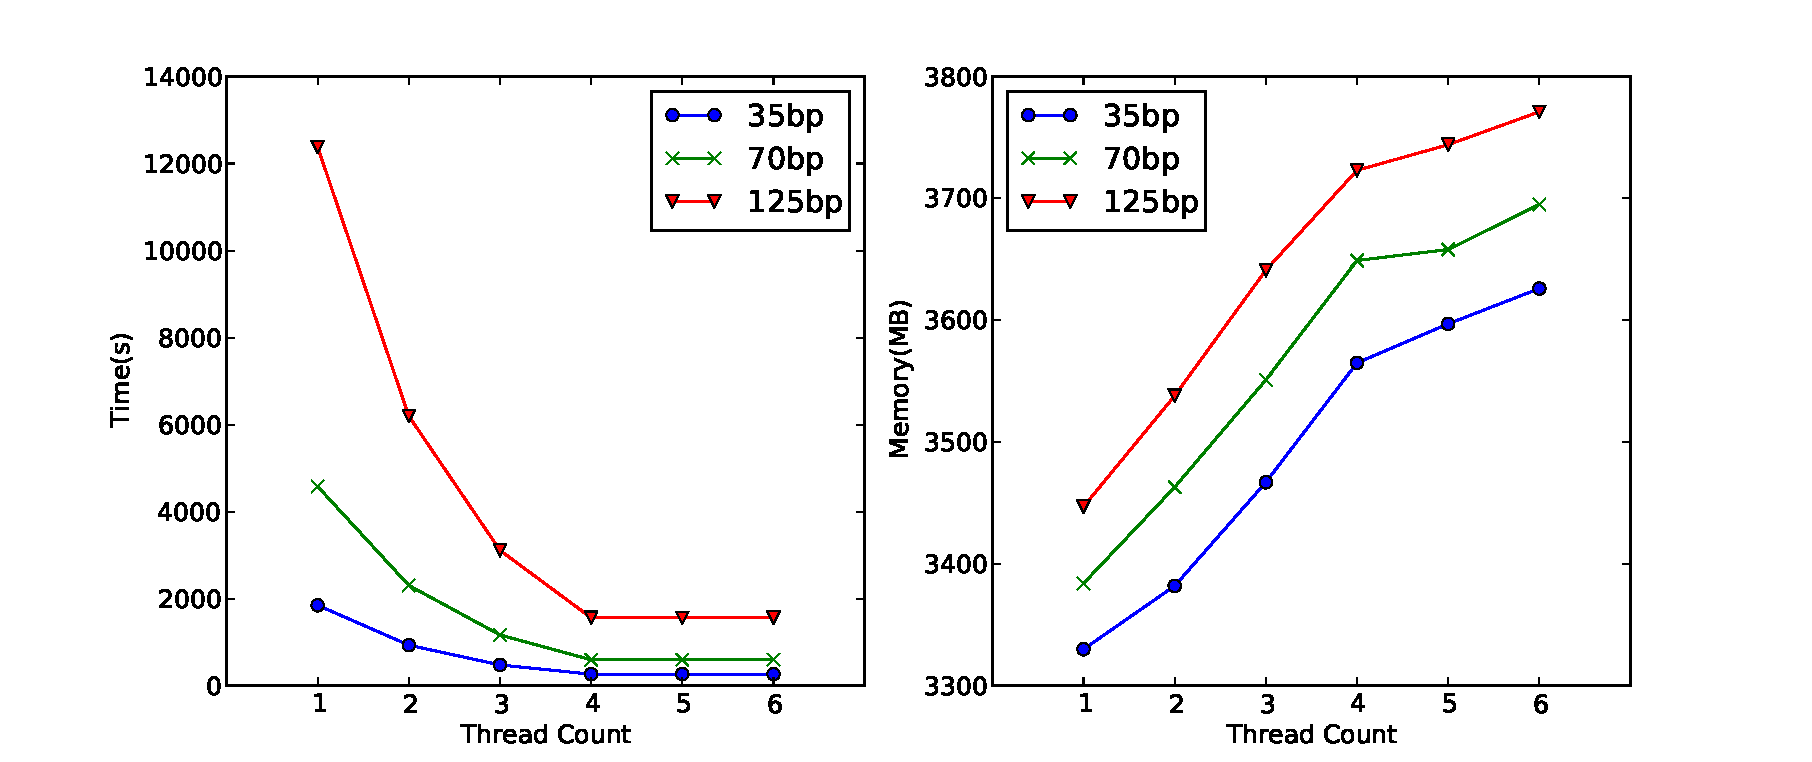
\includegraphics[width=1.1\textwidth]{alignment.pdf}
    \caption{多线程比对的时间空间效率} \label{fig:alignment}
\end{figure}

\section{使用seed提高比对速度}
在DNA测序技术中,单端测序和双端测序都存在测序质量的问题。离引物结合位点越近的位置,测序结果准确率越高,而越远的位置,测序准确率
越低。根据这一现象,关于Bowtie实现的论文\cite{langmead2009ultrafast}中提出了seed的概念,该论文认为针对短读序列中测序可信度较高
的部分采用较高的限制,在较低的地方做较低的限制可以取得更快的比对速度和更好的比对结果。如图\ref{fig:seed}所示,read前面绿色部分
是可信度比较高的seed部分,后面是可信度比较低的非seed部分。

\begin{figure}[htbp]
    \centering
    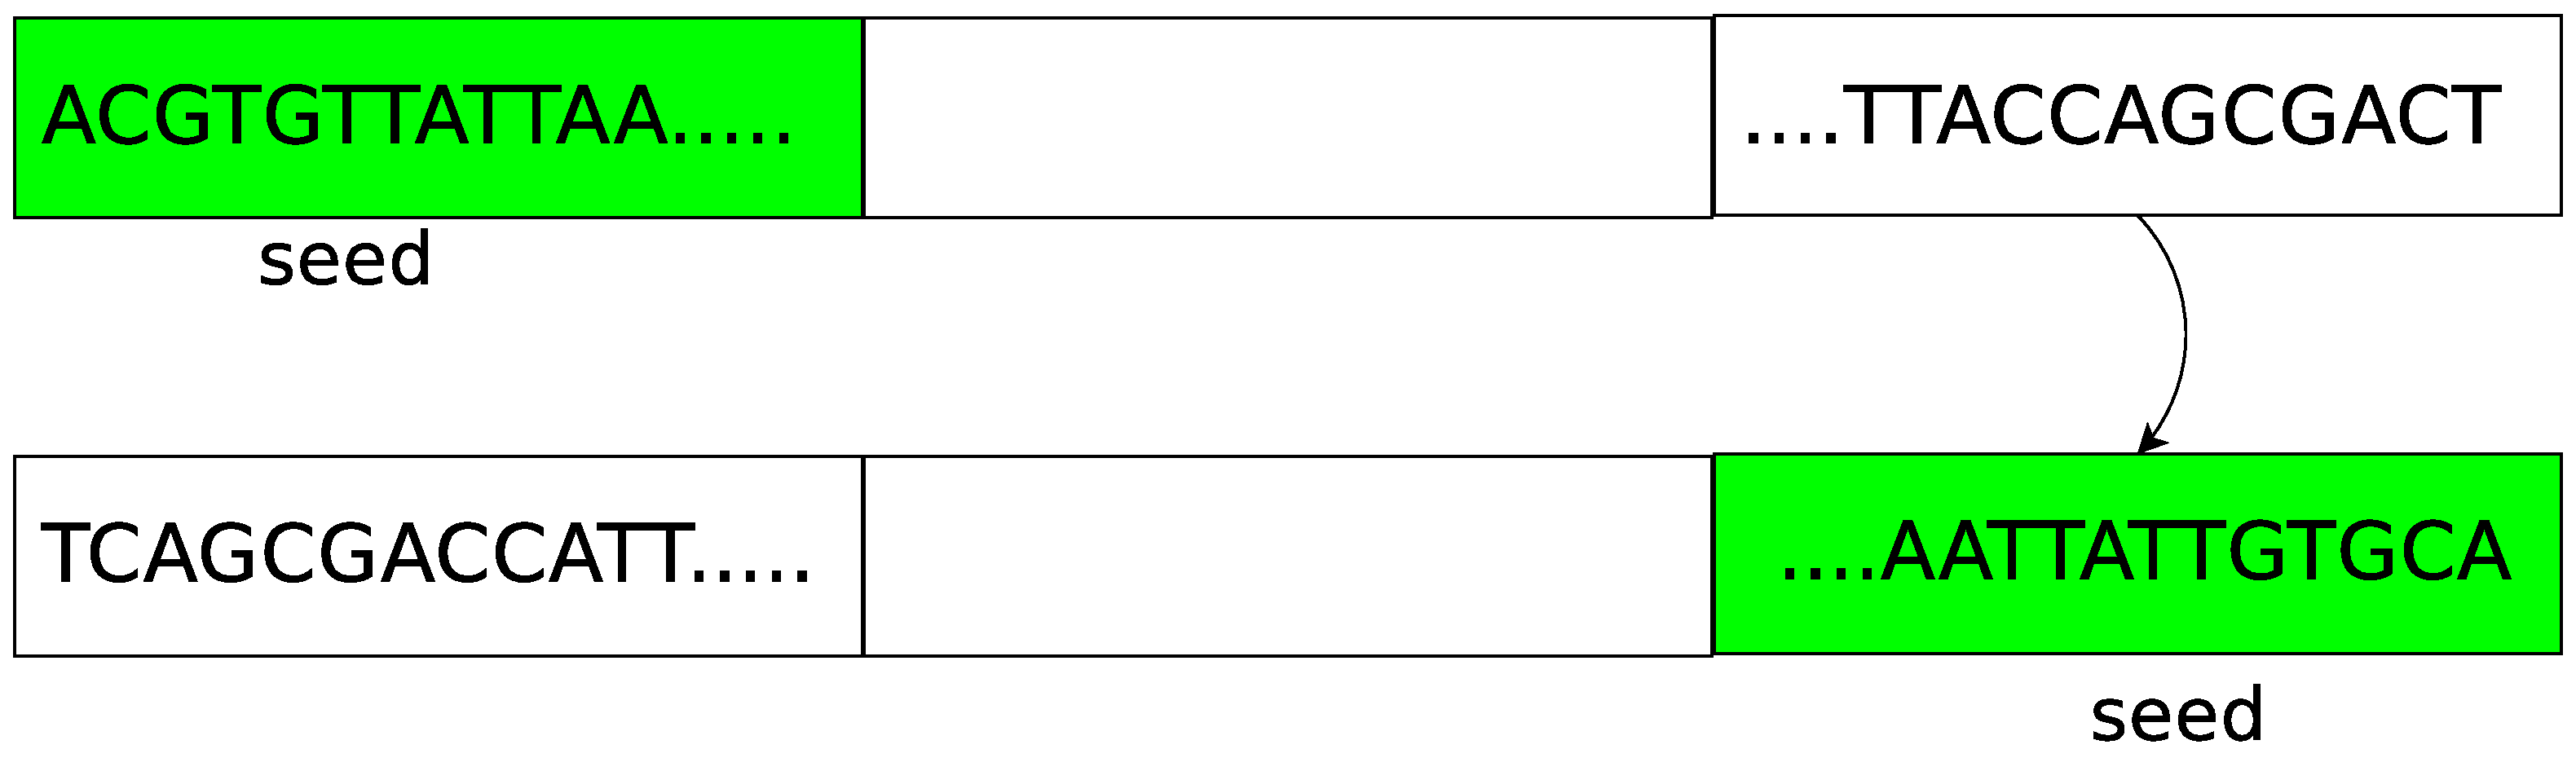
\includegraphics[width=0.9\textwidth]{seed.eps}
    \caption{seed示例} \label{fig:seed}
\end{figure}

在算法\ref{alg:alignment}中,我们当某个近似序列的$x.penalty>maxPenalty$时,会直接剪枝。CSAA中实际上是分为两部分来剪枝的,seed部有
一个$maxPenalty$,非seed部分有另一个$maxPenalty$,前者较小,后者较大。通过这样的策略,可以控制搜索结果中的待选近似序列中的替换
删除,插入等操作的绝大部分发生在非seed部分,即read的不可靠部分,从而有效提高比对的精度。至于seed的具体长度,可以根据不同的测序
技术来给定。默认情况下,Bowtie的seed长度是28,随本文发布的CSAA中seed的默认长度是32。

因为seed的限制条件较高,所以如果能首先对seed进行匹配,可以尽早抛弃掉一些不满足seed部分匹配要求,从而不用搜索非seed部分,从而
提高搜索速度。但因为seed是在短读序列的前缀部分,而我们使用CSA索引的后向搜索时是从后往前搜索的,最后才搜索seed部分。所以在CSAA中无论是建
立索引还是短读匹配都是对短读的逆序序列进行的。如图\ref{fig:seed}所示,通过逆序,把read的seed部分转到后向搜索的首先搜索的部分。

在图\ref{fig:seedaccuracy}中,对seed的长度对比对速度和比对精度做了对比测试,测试中的数据同图\ref{fig:alignment}使用的模拟数据相同,
都是100万条hg19上的仿真数据,indel概率为0.01\%,SNP概率为0.09\%,不同的是本次实验中只测试了长为70bp的短读。可以发现,seed的选
取对比对速度有着明显的影响,seed选取的越长,比对的速度越快,几乎成线性下降的趋势。seed的长度对recall rate和accuracy同样有影响,
seed选取的越长,recall rate有明显下降,这是因为如果seed越长,seed部分不匹配的可能越大,造成更多的短读不能匹配到参考序列上,而
accuracy有所提高则是因为较长的seed选取,抛弃了更多的可能错误匹配,保证了更少的匹配错误。

\begin{figure}[htbp]
    \centering
    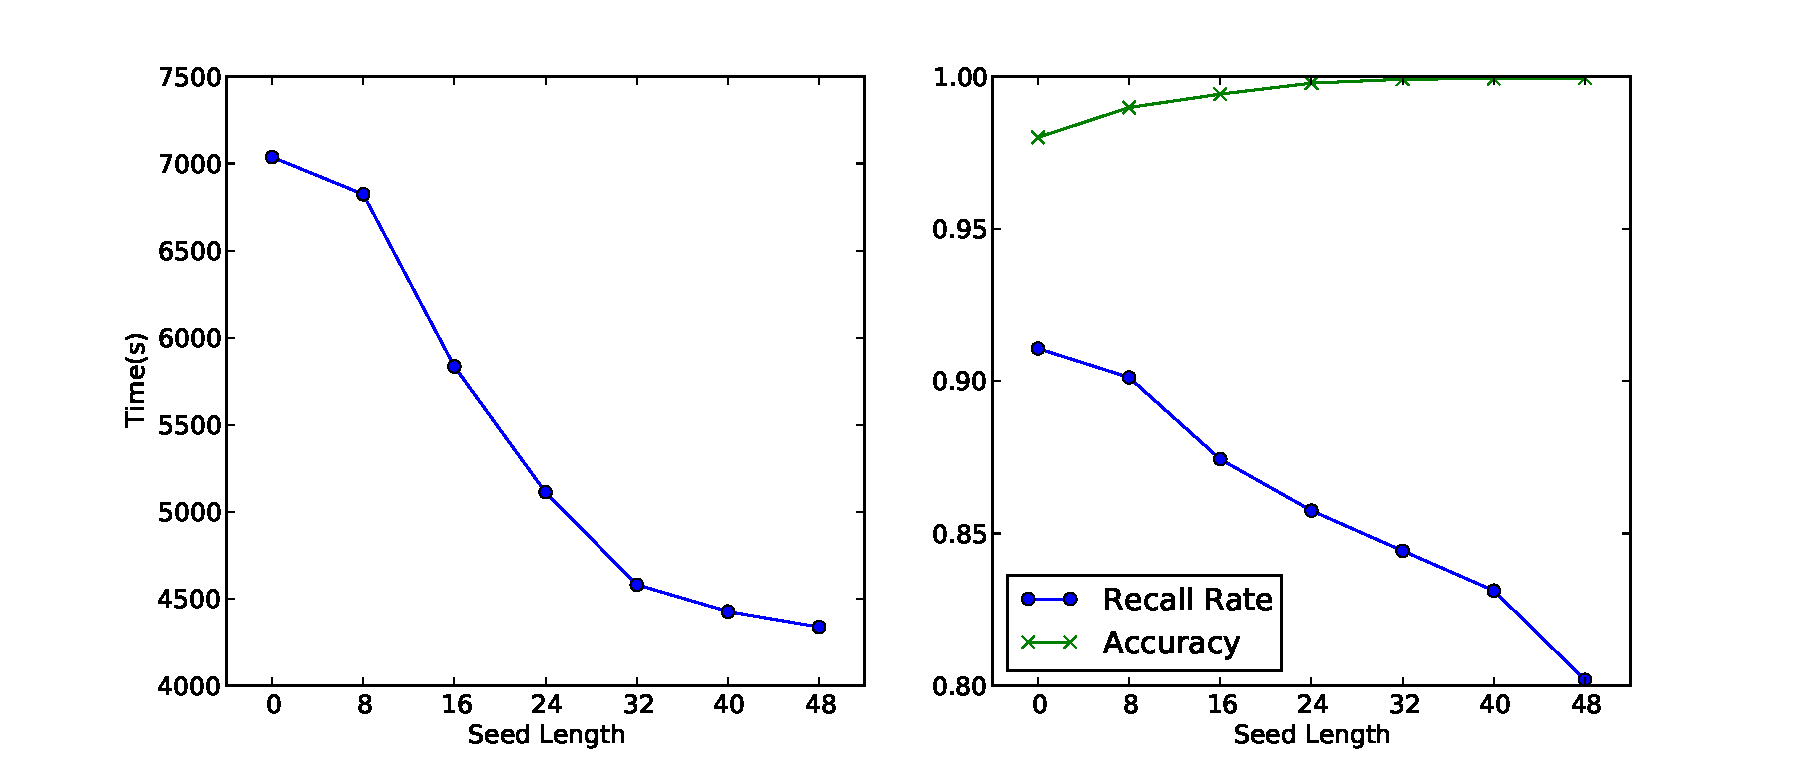
\includegraphics[width=1.1\textwidth]{seedaccuracy.pdf}
    \caption{seed长度对比对速度和比对精度的影响} \label{fig:seedaccuracy}
\end{figure}



本文中,比对精度包括两个测量指标,一个是recall rate,一个是mapping accuracy。recall rate是正确比对的短读(correctly mapped reads)
数占总的短读数(all reads)的比例,而mapping accuracy是正确比对的短读数(correctly mapped reads)占成功比对到参考序列上的短读(mapped reads)
的比例。在序列比对中,对于实际测序实验中得到的短读数据,由于预先并不知道短读的真正位置,所以正确比对的短读(correctly mapped reads)
数量是未知的。只有用模拟数据才能获取短读的真正位置,再用比对软件对模拟生成的短读进行比对,把获取的比对结果和预知的模拟短读的真正
位置做比较就能度量该比对软件的正确比对短读数目,从而计算出mapping accuracy,来度量一个软件的比对的可信度。另一方面,因为比对软件
在比对中设定的一些参数限制,如本文中的罚分,difference距离等等,使得一些发生了较大的变异(SNP,indels)的短读不能映射到参考序列上,
即该短读没有映射位置,从而造成最终在所有短读中只有一部分得以映射到参考序列上,这就是mapped reads,而recall rate即反映了这一衡
量短读比对性能的指标。在实际比对中,比对软件得到的参考序列上的比对位置和生成仿真数据时的实际位置并不需要完全比上,只要二者之间
的距离在一定距离内即认为这个比对结果是正确的,本文中所有的实验中这一距离定义为20。


\section{双端序列比对}
在前面的预备知识中我们提到了双端测序方法不同于单端测序,同一个fragment会得到两个read序列。CSAA可以支持双端数据的比对,比对的
算法和单端算法一致,分别对同一个个序列的reaed1和read2采用算法\ref{alg:alignment}进行比对,得到两个比对结果,最终使用合并程序
合并两个比对结果,得到最终比对结果。

如图\ref{fig:merge} phase3所示,双端测序时,因为测序精度的限制只能测序一个fragment的两端的部分数据,而大多数情况下因fragment比较
长两端的数据并不重合,所以read1和read2之间会有一个未测序的distance。。根据测序规则,序列都是从5'端开始读,因而read1和read2必然
是在DNA的不同链上,但测序时很难知道read1和read2是在DNA的某个具体链上,所以我们在比对时,需要把reaed1,read1的互补链,read2,
read2的互补连这四个序列分别和参考序列比对。但这样一来会导致需要比对四次,需要合并四个比对结果,合并的复杂度会很大。因此,CSAA
在实现时,采用了互补参考序列的方法,把参考序列和参考序列的互补序列的逆序列链接在一起,够成一个序列,从而减少了比对次数,如图
\ref{fig:merge}phase1到phase2所示。这样只需要比对两次即可,合并复杂度也降低了。

在合并read1和read2的比对结果时,CSAA除了比较两个比对结果集的比对得分之外,还通过比对distance来选定比对结果。如图\ref{fig:merge}
所示,途中phase3是一个虚拟的fragment到短读的测序示例,fragment长为10,双端测序的两个短读read1和read2都是4。通过比对程序,phase4
显示了比对的结果,可以看到,read1和read2都有两个最优的比对位置,read1的比对位置是$p1,p1'$,read2的比对位置是$p2,p2'$,由于$p2'>n$,
即该位置实在参考序列的互补链上,所以首先需要把$p2$转为参考序列的正确位置上,即$2n-p2'$,参考序列上该位置起从左向右的互补链是和
read2相匹配的。按照前文所述的双端测序方法可知,read1和read2是一个read2的两端的测序数据,所以比对的正确结果中,read1和read2的比对
位置之差应当为测序的fragment的长度,双端比对的两组比对结果合并的原则即检测比对的两组比对位置的差值
是否正好是fragment的长度,符合则该比对结果是可信的比对结果,不符合则抛弃。对应的在图\ref{fig:merge}中,可以发现$p1,p2'$这一组
比对结果才是合理的,因为$|(2n-p2')-p1|$正好是phase3中的fragment的长度。

在实际测序中,我们并不能能知道fragment的准确长度,而且经过分割,复制后的fragment的长度并不是长度都相等的,只能根据测序实验方法获
取一个范围,CSAA中,默认fragment长度为200到300之间,这是illumina实验的fragment长度范围。

\begin{figure}[htbp]
    \centering
    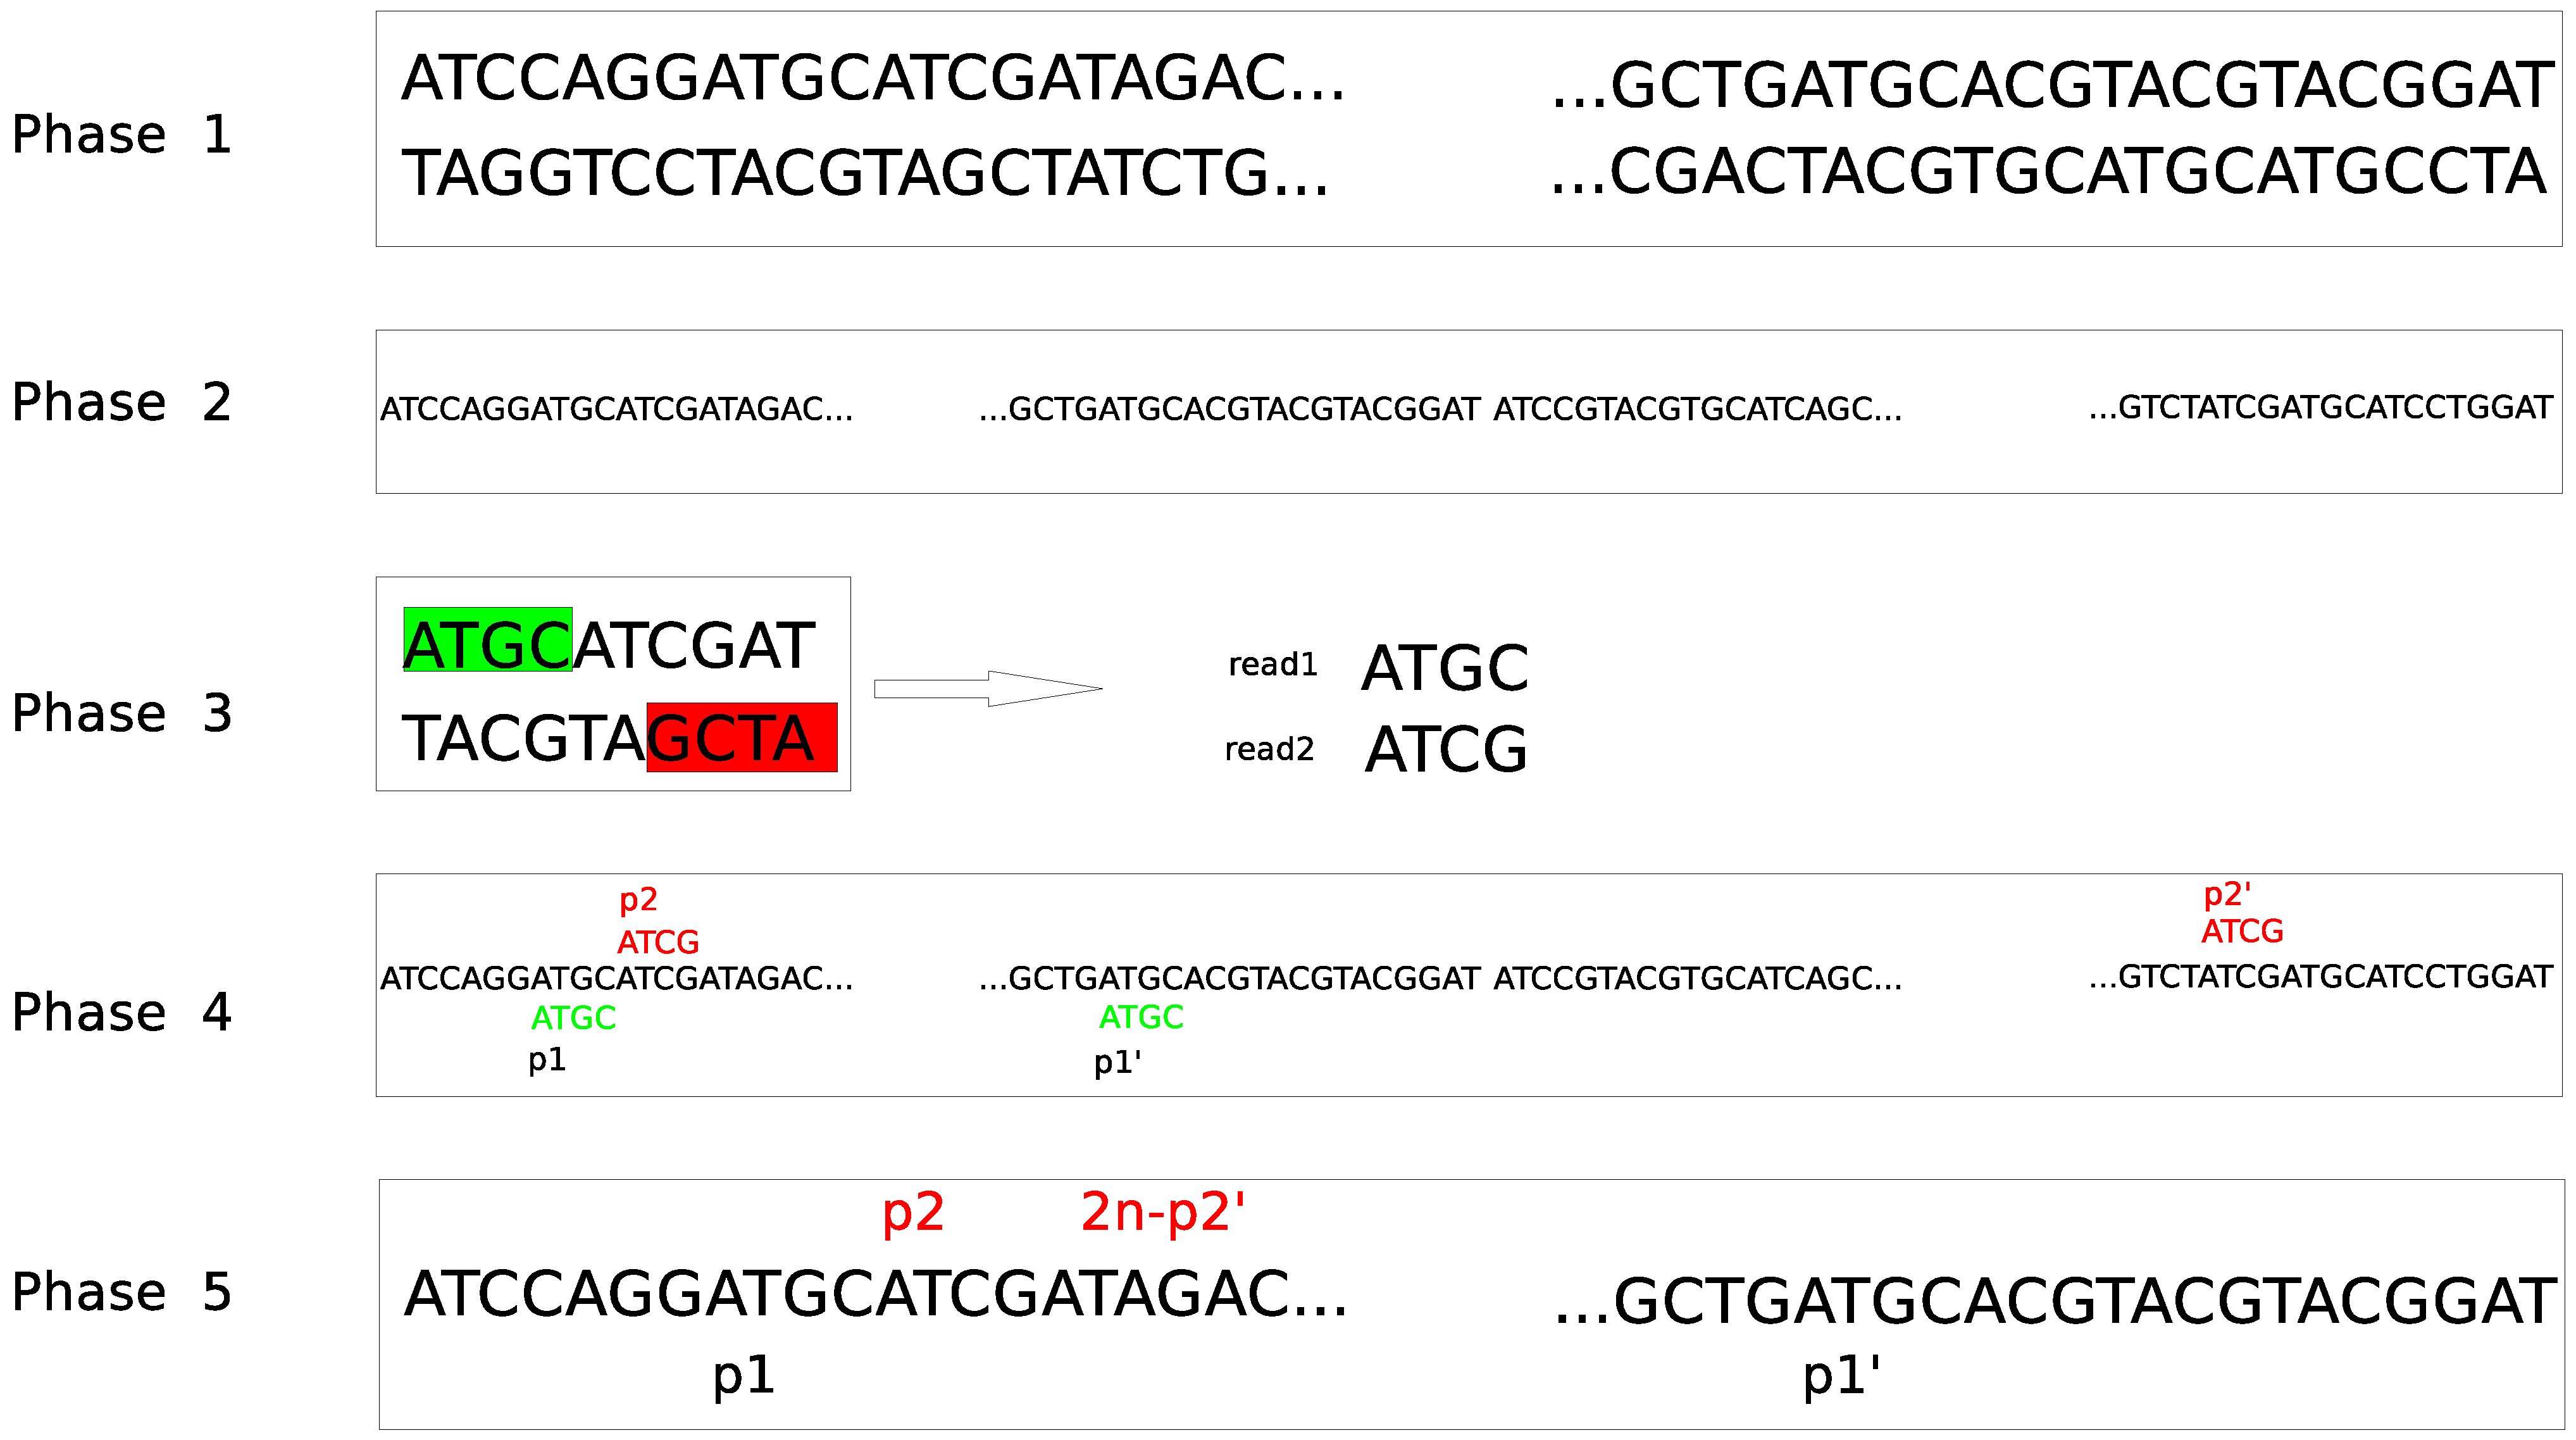
\includegraphics[width=0.95\textwidth]{merge.eps}
    \caption{双端比对示例} \label{fig:merge}
\end{figure}

综上所述,在CSAA中用双端比对可以提高比对的精度,表\ref{tab:alignmentaccuracy}也反映了这点,但对应的双端比对要耗费更多的时间,是
单端比对的两倍时间多。表\ref{tab:alignmentaccuracy}使用的数据和图\ref{fig:seedaccuracy}中使用的数据相同,比对过程都使用单线程。

\begin{table}[htbp]
    \caption{单端比对和双端比对结果对比}
    \label{tab:alignmentaccuracy}
    \centering
    \begin{tabular}{lrrrp{2ex}rrr}
        \toprule
        \multirow{2}{*}{短读长度} & \multicolumn{3}{c}{单端比对}& & \multicolumn{3}{c}{双端比对}\\
        \cline{2-4}
        \cline{6-8}
        &Time(m) &Rec(\%) &Acc(\%)& &Time(m) &Rec(\%) &Acc(\%)\\
        \midrule
        35 &3.35 &80 &98.1& &8.0 &88.4 &98.2 \\
        70 &7.67 &84 &98.1& &16.85 &92.2 &98.2 \\
        125 &17.85 &87 &98.3& &36.87 &94.1 &98.4 \\
        \bottomrule
    \end{tabular}
\end{table}



\section{CSAA对比实验测试}

为测试CSAA的性能,本文同时测试了Bowtie\cite{langmead2009ultrafast}和BWA\cite{li2009fast}这两个个比对工
具的性能,以和CSAA进行比较。分别对比这几个工具在不同规模数据上建立索引时的时间,需要的内存;以及在模拟数据上和真实数据上的比对能力。
这三个工具中,Bowtie和BWA是用基于BWT的索引建立
的比对工具,其中Bowtie采用了回溯法实现替换操作,但不支持insert和delete操作,即上文中所论述的gap alignment。BWA除了支持insert,
delete之外,还加入了smith-water方法提高比对精度。此外Bowtie和BWA和我们的CSAA都支持多线程比对,但在比对测试中,我们的csaa和bwa,
bowtie等都只使用单线程运行。

\subsection{测试环境和数据}

在对CSAA的对比测试中,我们使用gcc 4.8编译链接CSAA,并且使用了-O3优化。系统环境为ubuntu 12.04 amd64,运行在一台具有18G内存和双
核intel Xeon(R) CPU的工
作站上。测试使用的数据是标准的人类基因组序列,ucsc version为hg19,来自1000 Genome Project的名为Genome Reference Consortium GRCh37
的参考序列。实验中所用的模拟数据也是在该数据上生成。

测试中,CSAA和BWA在测试时均指定单线程,seed长为32。Bowtie使用的是Bowtie-v1,使用单线程,且不使用-best参数,即Bowtie使用DFS搜索。
Bowtie使用默认的长为31的seed。模拟数据的获取和比对精度结果获得中使用了SAMtools系列工具中的wgsim和wgsim-eval。

\subsection{索引建立时间}
表\ref{tab:tab1}中对比了bowtie,BWA和CSAA三种工具分别建立索引时所需要的时间和内存消耗对比情况,表中数据分别对应几个工具在索引
512M,1024M和2048M的数据时所需要的时间和内存。CSAA中使用经典方法构建压缩后缀数组。

\begin{table}[htbp]
    \caption{建立索引的时间空间对比}
    \label{tab:tab1}
    \centering
    \begin{tabular}{lrrrp{2ex}rrr}
        \hline
        \multirow{2}{*}{Program} & \multicolumn{3}{c}{Time(m)}& & \multicolumn{3}{c}{Memory(MB)}\\
        \cline{2-4}
        \cline{6-8}
        & 512M &1024M &2048M& &512M &1024M &2048M\\
        \hline
        Bowtie&21.85 &45.33 &93.02& &987 &1109 &1210 \\
        BWA&7.85 &16.33 &34.72& &1890 &1902 &2006 \\
        CSAA&6.27 &14.0 &29.87& &2113 &8680.1 &19532.5 \\
        \hline
    \end{tabular}
\end{table}

从表\ref{tab:tab1}中的测试结果可以看到,CSAA相对其他两个不对工具在索引时间上具有较大优势,这是由于BWA和Bowtie都同时给inverted
reference建立了索引,用时会较长。其中Bowtie建立索引时是分块建立索引的,最终再合并成一个索引,时间效率最差,但需用内存空间最小。

\subsection{模拟数据测试}
本文使用SAMtools工具包中的wgsim工具从人类基因组序列hg19中随机生成模拟的短读序列。然后,分别用四种比对工具对这些模拟的
短读序列进行比对,最后测试比对速度以及比对精确度。因为这些模拟数据在参考序列上的映射位置是已知的,所以可以计算出各个工具的比
对结果的accuracy。本次实验中的精度测试工具使用SAMtools中的wgsim\_eval.pl程序。

表\ref{tab:singleend}和\ref{tab:pairend}所示为四个测试工具在单端和双端模拟数据上的的比对结果展示,参考序列是人类基因组序列
hg19,模拟短读序列的长度为70bp,总共有100万个短读。

表\ref{tab:singleend}和\ref{tab:pairend}中的实验的模拟数据使用wgsim程序在人类基因组上生成的长为70bp,生成过程中,单核苷酸变
异(SNP)的概率是0.09\%,indel变异的概率是0.01\%,生成双端模拟数据时的fragment distance的长度满足正太分布$N(500,50)$。对比结果中Rec是recall rate,Acc是accuracy。
意义如上文中所解释。从表中可以看出,在长为70bp的100万个短读的映射中,CSAA相对于BWA和Bowtie在查询时更节省内存,在recall rate和
accuracy上和BWA,Bowtie基本持平。%出现这样的结果是因为BWA和CSAA都支持indel操作,而Bowtie则只支持substitution操作,当短读序列比
%较长时其比对效果就会下降。


\begin{table}[htbp]
    \caption{单端模拟数据比对测试}
    \label{tab:singleend}
    \centering
    \begin{tabular}{lrrrr}
       \toprule \\
       Program&Time(m)&Memory(M)&Rec(\%)&Acc(\%)\\
       \midrule \\
       Bowtie&10.2&2911&85.3&99.8\\
       BWA&7.8&3116&90.7&99.8\\
       CSAA&8.9&2905&84&98.1\\
       \bottomrule
    \end{tabular}
\end{table}


\begin{table}[htbp]
    \caption{双端模拟数据比对测试}
    \label{tab:pairend}
    \centering
    \begin{tabular}{lrrrr}
       \toprule \\
       Program&Time(m)&Memory(M)&Rec(\%)&Acc(\%)\\
       \midrule \\
       Bowtie&10.05&3011&89.6&99.2\\
       BWA&13.7&3117&94.3&99.8\\
       CSAA&16.85&2905&92.2&98.2\\
       \bottomrule
    \end{tabular}
\end{table}

\subsection{真实数据测试}
为测试CSAA在真实数据上的表现,本文从网络上下载了12.2 million个长为51bp的短读数据库。这些数据来自European Read Archive
(AC:ERR000589),是1000 Genomes Project的一个名男性基因组测序,由Illumina测序技术完成测序。参考序列选的是人类基因组,
测序编号hg19。由于真实数据的比对位置并不能事先获取,所以在测试真实数据时使用Mapped rate来度量比对效果。Mapped rate
指比对程序在指定参数条件下能够给出比对结果的短读数目和所有测试数据中短读数目总和的比例。在本次比对中测试中,BWA,CSAA,
Bowtie和MAQ都是单线程比对,BWA和CSAA使用默认的长为32的seed策略,Bowtie使用长为31的seed策略,Maq使用-n 2参数,指定最大
允许的mismatch数目为2。

\begin{table}[htbp]
    \caption{实际数据比对测试}
    \label{tab:tab3}
    \centering
    \begin{tabular}{lrrr}
       \toprule
       Program&Time(m)&Memory(MB)&Mapped(\%)\\
       \midrule
       Bowtie&53&3122&84.6\\
       BWA&62&3887&88.4\\
       CSAA&87&3413&84.5\\
       MAQ&647&4824&86.4\\
       \bottomrule
    \end{tabular}
\end{table}

表\ref{tab:tab3}中的测试结果显示,在实际数据中CSAA也具有较高的准确性,84\%的短读序列都能映射到参考序列上,
基本性能和BWA很接近。在时间方面,CSAA,BWA,Bowtie都使用索引参考序列再比对的方法,而MAQ则使用了索引短读序列的方法,所以
CSAA,BWA,Bowtie的比对时间都比较接近,Bowtie能更快一些。在比对使用的空间上,相对而言,CSAA使用了更少的内存,空间效率
优于其他三种发放,在常规PC机上具有优势。

\section{本章小节}

本章主要介绍了CSAA在实现方面所做的一些优化,以及相应的优化的实验效果展示。本章首先在第一节介绍了改进后的压缩后缀数组索引算法
在空间方面的效率。第二节主要介绍采用并行化方法提高比对效率的方法和效果。第三节介绍seed的概念以及采用seed提高比对精确度的方法。
第四小节紧接着描述了CSAA对双端测序的支持。最后一小节通过综合比对测试,对比CSAA和常见的几种比对程序的比对效果,可以看到CSAA在
比对精度和时间上还是有很大的优势的。

    
\chapter{总结与展望}
\label{chap:con}

\subsection{总结}

\subsection{进一步工作}

%    \appendix
%    
\chapter[本科生毕业设计论文撰写规范]{西安电子科技大学本科生毕业设计论文撰写规范}
\label{chap:requires}
\section{毕业设计(论文)的总体要求}
撰写论文应简明扼要,一般不少于15000字(外语专业可适当减少,但不得少于10000单词,且须全部用外语书写)。

\section{毕业设计(论文)的编写格式}
每一章、节的格式和版面要求整齐划一、层次清楚。其中:
\begin{itemize}
  \item 论文用纸:统一用A4纸,与论文封皮,任务书,工作计划,成绩考核表一致。
  \item 章的标题:如:``摘要''、``目录''、``第一章''、``附录''等,黑体,三号,居中排列。
  \item 节的标题:如:``2.1  认证方案''、``9.5  小结''等,宋体,四号,居中排列。
  \item 正文:中文为宋体,英文为``Times News Roman'',小四号。正文中的图名和表名,宋体,五号。
  \item 页眉:宋体五号,居中排列。左面页眉为论文题目,右面页眉为章次和章标题。页眉底划线的宽度为0.75磅。
  \item 页码:宋体小五号,排在页眉行的最外侧,不加任何修饰。
\end{itemize}

\section{毕业设计(论文)的前置部分}
毕业设计(论文)的前置部分包括封面、中英文摘要、目录等。
\subsection{封面及打印格式}
\begin{itemize}
  \item 学号:按照学校的统一编号,在右上角正确打印自己的学号,宋体,小四号,加粗。
  \item 题目:题目应和任务书的题目一致,黑体,三号。
  \item 学院、专业、班级、学生姓名和导师姓名职称等内容,宋体,小三号,居中排列。
\end{itemize}

\subsection{中英文摘要及关键词}
摘要是关于论文的内容不加注释和评论的简短陈述,具有独立性和自含性。它主要是
简要说明研究工作的目的、方法、结果和结论,重点说明本论文的成果和新见解。关键词
是为了文献标引工作从论文中选取出来用以表示全文主题内容信息的术语。
\begin{enumerate}
  \item 中文摘要,宋体小四号,一般为300字;英文摘要,``Times News Roman''字
体,小四号,一般为300个实词。摘要中不宜出现公式、非公用的符号、术语等。
  \item 每篇论文选取3 \~{} 5个关键词,中文为黑体小四号,英文为``Times News Roman''字体加粗,小四号。关键词排列在摘要的左下方一行,起始格式为:``\textbf{关键词}:
      ''和``\textbf{Keyword:}''。具体的各个关键词以均匀间隔排列,之间不加任何分隔符号。
\end{enumerate}

\section{目录}
按照论文的章、节、附录等前后顺序,编写序号、名称和页码。目录页排在中英文摘要之后,主体部分必
须另页右面开始,全文以右页为单页页码。

\section{毕业设计(论文)的主体部分}
毕业设计(论文)的主体部分包括引言(绪论)、正文、结论、结束语、致谢、参考文献。
\subsection{绪论}
作为论文的开端,简要说明作者所做工作的目的、范围、国内外进展情况、前人研究成果、
本人的设想、研究方法等。
\subsection{正文} 为毕业设计(论文)的核心部分,包括理论分析、数据资料、实验方法、结果、本人的论点和结
论等内容,还要附有各种有关的图表、照片、公式等。要求理论正确、逻辑清楚、层次分明、文字流畅、数据真实可
靠,公式推导和计算结果无误,图表绘制要少而精。
\begin{description}
  \item[图] 包括曲线图、示意图、流程图、框图等。图序号一律用阿拉伯数字分章依序编码,如:图1.3、图2.11。每一图应有简短确切的
      图名,连同图序号置于图的正下方。图中坐标上标注的符号和缩略词必须与正文中一致。
  \item[表] 包括分类项目和数据,一般要求分类项目由左至右横排,数据从上到下竖列。分类项目横排中必须标明符号或单位,竖列的数据栏中不宜出现``同上'' 、``同左''等类似词语,一律填写具体的数字或文字。表序号一律用阿拉伯数字分章依序编码,如:表2.5、表10.3。每一表应有简短确切的题名,
      连同表序号置于表的正上方。
  \item[公式] 正文中的公式、算式、方程式等必须编排序号,序号一律用阿拉伯数字分章依序编码,如:式(3-32)、式(6-21)。对于较长的公式,另行居中横排,只可在符号处(如:+、-、*、/、$<$、 $>$等)转行。公式序号标注于该式所在行(当有续行时,应标注于最后 一行)的最右边。连续性的公式在``=''处排列整齐。大于999的整数或多于三位的小数,一律用半个阿拉伯数字符的小间隔分开;小于1的数应将0置于小数点之前。
  \item[计量单位] 单位名称和符号的书写方式一律采用国际通用符号。
\end{description}

\subsection{结论}
是对主体的最终结论,应准确、完整、精炼。阐述作者创造性工作在本研究领域的地位和作用,对存在的问题和不足应给予客观的说明,也可提出进一步的设想。

\subsection{致谢}
对协助完成论文研究工作的单位和个人表示感谢。

\subsection{参考文献}
在学位论文中引用参考文献时,引出处右上角用方括号标注阿拉伯数字编排的序号(必须与参考文献一致)。参考文献的排列格
式分为:
\begin{description}
  \item[专著类的文献] [序号]  作者 . 专著名称.  版本. 出版地:出版者,出版年. 参考的页码。
  \item[期刊类的文献] 作者 . 文献名. 期刊名称.  年 , 月,  卷(期). 页码。
\end{description}
其中作者采用姓在前、名在后的形式。当作者超过三个时,只著录前三个人,其后
加``等''字即可。

\section{毕业设计(论文)的附录部分}
附录是作为学位论文主体的补充,包括下列内容:
\begin{enumerate}
  \item 正文中过于冗长的公式推导;
  \item 为读者阅读方便所需要的辅助性的数学工作或带有重复性的图表;
  \item 由于过分冗长而不宜在正文中出现的计算机程序清单;
  \item 对于一般读者并非必要阅读,但对本专业同行有参考价值的资料。
  \item 附录编于正文后,与正文连续编页码,每一附录均另页起。
  \item 附录依次用大写正体A,B,C……编序号,黑体,三号。如:附录A。
  \item 附录中的图、表、式、参考文献等与正文分开,用阿拉伯数字另行编序号,注意在数码前冠以附录的
      序码。如:图A1;表B2;式(C-3);文献[D5]。
\end{enumerate}
\section{毕业设计(论文)的打印规格}
论文正文页面和版面的设置规格:论文正文双面打印,为了便于装订、复制,要求每页纸的四周留有足够的空白边缘。以WORD97为例:

页面设置数据为:上3厘米、下2厘米、内侧3厘米、外侧2厘米;装订线 -- 1厘米;页眉  - 2厘米;  页脚 - 1厘米。

版面设置数据为:文字的行间距 - 1. 5倍 ;  公式的行间距 - 1. 5倍字符间距 - 标准;页码数据-对称页边距。

\section{毕业设计(论文)的装订说明}
毕业设计(论文)要求以A4纸的标准,按照下列顺序装订。外文资料翻译原文及译文另册装订,格式参照论文对应内容格式要求。

\begin{enumerate}
  \item 封面
  \item 任务书
  \item 工作计划
  \item 中期检查表
  \item 成绩考核登记表
  \item 中、外论文摘要
  \item 目录
  \item 引言
  \item 论文
  \item 结论
  \item 结束语
  \item 参考文献
  \item 附录
\end{enumerate}












%%----------------- 附件部分 ----------------- %%
    \backmatter
    %\include{chapter-utf8/bib1}
    \bibliography{reference}
    
\begin{thanks}

毕业论文暂告收尾,这也意味着我在西安电子科技大学的四年的学习生活既将结束。
回首既往,自己一生最宝贵的时光能于这样的校园之中,能在众多学富五车、才华
横溢的老师们的熏陶下度过,实是荣幸之极。在这四年的时间里,我在学习上和思
想上都受益非浅。这除了自身努力外,与各位老师、同学和朋友的关心、支持和鼓
励是分不开的论文的写作是枯燥艰辛而又富有挑战的。

数学是理论界一直探讨的热门话题,老师的谆谆诱导、同学的出谋划策及家长的支持
鼓励,是我坚持完成论文的动力源泉。在此,我特别要感谢我的导师xxx老师。从论文
的选题、文献的采集、框架的设计、结构的布局到最终的论文定稿,从内容到格式,
从标题到标点,她都费尽心血。没有xxx老师的辛勤栽培、孜孜教诲,就没有我论文
的顺利完成。

感谢数学系的各位同学,与他们的交流使我受益颇多。最后要感谢我的家人以及我的
朋友们对我的理解、支持、鼓励和帮助,正是因为有了他们,我所做的一切才更有意
义;也正是因为有了他们,我才有了追求进步的勇气和信心。

时间的仓促及自身专业水平的不足,整篇论文肯定存在尚未发现的缺点和错误。
恳请阅读此篇论文的老师、同学,多予指正,不胜感激!
......

\vskip 18pt

谨把本文献给我最敬爱的父母亲以及所有关心我的人!

\end{thanks}

    \begin{authorintro}

{
    \bf\songti\zihao{5}
    \noindent
    1. 基本情况
}

男,陕西省商洛市人,1989年10月出生,西安电子科技大学计算机学院计算机软件与理论专业2012级硕士研究生。

{
    \bf\songti\zihao{5}
    \noindent
    2. 教育背景
}

2008.08~2012.07\quad\quad 就读于西安电子科技大学计算机学院计算机科学与技术专业,获得工学学士学位

2012.08~\hspace{2.2cm}       西安电子科技大学计算机学院计算机软件与理论专业硕士研究生



{
    \bf\songti\zihao{5}
    \noindent
    3. 在学期间的研究成果
}

\end{authorintro}
1.“大数据压缩索引及搜索算法研究”,国家自然科学基金



\end{document}



